%-------------------------------------------------------------------------
%	Lecture Notes Stochastic Processes, Benjamin Wolba
%-------------------------------------------------------------------------

\documentclass{notebook}

\ihead{\headmark}													  % header: chapter name inside
\setheadsepline{0.5pt}												% insert line of 0.5 pt width
\cfoot{Made with \LaTeX{} by Benjamin Wolba}
	
\addbibresource{ref.bib} 										   % integration of .bib-file

\newcommand{\blue}[1]{{\color{bluebase}#1}}

\title{\color{bluebase} Lecture Notes on Stochastic Processes}  
\author{Prof. Dr. Benjamin M. Friedrich, Dr. Benjamin Wolba}                 

% Style Guide 
% 
% - concepts, definitions, theorems, etc. go inside a "theorem" environment
% - remarks, comments, digressions go inside a "remark" environment 
% - new technicals terms should be introduced for the first time in italics
% ... 
% 


\begin{document}
	
\frontmatter

\maketitle

\tableofcontents

\mainmatter

\chapter{Prerequisites: Probability Theory}

\section{Mathematical Foundations}

\begin{theorem}[Concept: Probability]
	%
	Let $X$ be a set of states, then we have the following axioms of probability:
	%
	\begin{itemize}
		\item{$P(A)$ is a function with $0 \leq P(A) \leq 1$ defined for every `nice' subset $A \subseteq X$}
		\item{Additivity: $P(A) + P(B) = P(A \cup B) - P(A \cap B)$}
	\end{itemize}
	%
\end{theorem}

Example 1: fair coin: $X=\{\text{head},\text{tail}\}$, $P(\{\text{head}\})=1/2$, 
(we will often use sloppy notation $p(\text{head})$ for sets $A$ with single element only)\\
Example 2: perfect dice: $X=\{1,2,3,4,5,6\}$, $P(\{1,2\})=P(1)+P(2)=1/3$

If $X = \R$, we can consider a \textit{probability density} 
as a function $p(x) : \R \to \R^+$, which relates to the probability by
%
\begin{equation}
\label{eq:def_P}
P(A) = \int_A{\dd{x} p(x)}
\end{equation}
%
for $A \subseteq \R$. 

Note that $p(x)$ is also called \textit{probability density function} 
and sometimes written as $\mathrm{PDF}(x) = p(x)$. 
Also, note the physical units: 
if, for example, $x$ has units of a length, $[x] = \si{\meter}$, 
then the probability density $p(x)$ has units of an inverse length, $[p] = \si{\per \meter}$. 
Knowing the physical units allows to tell apart different objects.

As a mathematical caveat, Eq.~\eqref{eq:def_P} cannot be defined for arbitrarily ``wild'' sub-sets $A \subset \R$, but only for sufficiently `nice' subsets. Specifically, these subsets need to be measurable and thus form a so-called $\sigma$-algebra. This technical issue is extensively studied in the mathematical sub-discipline of measure and integration theory, but usually is not a concern in physical applications.
In particular, (countable) unions and intersections of intervals are measurable.
For a reference, see e.g. \cite{Billingsley2012}.


The \textit{cumulative density function} is defined as
%
\begin{equation}
\mathrm{CDF}(x) = \int^x_{-\infty}{\dd{x'} p(x')}
\end{equation}
%
Important characteristics of probability distributions are there moments and its cumulants.

\begin{theorem}[Moments]
	%
	The \textit{moments} of a probability distribution $p(x)$ are defined as
	%
	\begin{equation}
	\mu_n = \expval{x^n} = \int^{\infty}_{-\infty}{x^n p(x)}
	\end{equation}
	%
	with the characteristic function
	%
	\begin{equation}
	\label{eq:def_moment}
	\expval{\exp(t x)} = \sum^{\infty}_{n = 0}{\mu_n \frac{t^n}{n!}}\quad,
	\end{equation}
	%
	i.e., the moments are the Taylor coefficients of the characteristic function
\end{theorem}

\begin{theorem}[Cumulants]
	%
	The \textit{cumulants} are given by the mean value $k_1 = \mu_1$, the variance $k_2 = \mu_2 - \mu^2_1$ and higher order cumulants such as $ k_3 = \mu_3 - 3 \mu_2 \mu_1 + 2 \mu_1^3$. More generally we have
	%
	\begin{equation}
	\label{eq:def_cumulant}
	\ln \expval{\exp(t x)} = \sum^{\infty}_{n = 0}{k_n \frac{t^n}{n!}}
	\end{equation}
	%
\end{theorem}

Remark: Moments and cumulants contain the same information:
by inserting for example Eq.~(\ref{eq:def_cumulant}) into the Taylor series of the exponential function, 
and collecting equal powers of $t$ (after applying the binomial formula to expand powers), one obtains complicated formulas expressing the $n$th moment $\mu_n$ in terms of all $k_k$, $k\le n$.
A series of moments ``almost'' uniquely determines the underlying probability density function $p(x)$
(yet there are some mathematical delicacies for which we refer the reader to the mathematics literature
% TODO reference to literature should be added here
). 
Often, moments can be computed more directly, while cumulants allow to read off relevant information more readily.

Remark: For some probability distributions (e.g., probability distributions with polynomial tails, also called `fat tails'), higher moments may be infinite.

Example: For the normal distribution with mean $\mu$ and variance $\sigma^2$, we have 
$k_0 = \mu_0=1$ (this is just the normalization condition), 
$k_1=\mu_1=\mu$ (mean), 
$k_2=\mu_2-\mu_1^2=\sigma^2$ (variance), as well as $k_k=0$ for $k \ge 3$.
Conversely, a probability distribution whose higher cumulants vanish, 
i.e., $k_k=0$ for $k \ge 3$, is necessarily a normal distribution.


\section{Probability in Physics}

Usually, probability is regarded as relative frequency of an event $A$ occurring $N_A$ times while the total number of measurements is $N$
%
\begin{equation}
P(A) = \lim_{N \to \infty}{\frac{N_A}{N}}
\end{equation}
%
Practically, a probability is determined by
%
\begin{itemize}
	\item{the experiment being repeated very often with the same initial macrostate}
	\item{replacing the physical system by an idealized model for stochastic simulations}
\end{itemize}
%
(Talk by Jan Nagel: Gott würfelt nicht. Oder doch? (https://youtu.be/q-ezpVF6cL4) --> Uncertainty in initial conditions leads to a dice producing a stochastic behavior.)

\subsection*{Example Weather Forecast}

For an event R $=$ "rain tomorrow" we know that it is raining 116 out of 365 days in Dresden: $P(R \, | \, \mathrm{Dresden}) = \frac{116}{365} = 18 \%$. Our forecast is getting more accurate if we consider also seasonal changes and thus specify the month being October with 8 days of rain out of 31 in total: $P(R \, | \, \mathrm{Dresden, October}) = \frac{8}{31} = 25.8 \%$

Another approach is based on persistence of conditions, i.e. to make a rain prediction for tomorrow based on the weather today. E.g. according to Caskey 1963 we have $P(R \, | \, \mathrm{current \, local \, weather}) = x$ and $P(R \, | \, \mathrm{rain \, today}) = 44 \%$, $P(R \, | \, \mathrm{dry \, today}) = 17 \%$

Last but not least we can sample macrostates that are consistent with measurement data and calculate the probabilities for rain from deterministic models (Navier-Stokes-equations / mathematical forecasting) $P(R \, | \, \mathrm{current \, global \, weather})$.

\section{Important Probability Distributions}

\subsection*{Normal Distribution}

The normal distribution $N(\mu, \sigma^2)$ with mean $\mu$ and variance $\sigma^2$ is given by
%
\begin{equation}
p(x) = \frac{1}{\sqrt{2 \pi \sigma^2}} \exp[- \frac{(x- \mu)^2}{2 \sigma^2}] = N(\mu, \sigma^2)
\end{equation}
%
The moments and cumulants read
%
\begin{gather*}
	\mu_1 = \mu, \, \mu_2 = \mu^2 + \sigma^2, \, \mu_3 = \mu^3 + 3 \mu \sigma^2 \\
	k_1 = \mu, \, k_2 = \sigma^2, \, k_j = 0 \quad \mathrm{for} \quad j \geq 3
\end{gather*}
%

\subsection*{Bernoulli Distribution}

For a Bernoulli trial you have two outcomes with respective probabilities $p$ and $1 - p$. If you now perform $n$ independent trials you will get $k$ times the first outcome with probability
%
\begin{equation}
P(k,n) = \binom{n}{k} p^k (1 - p)^{n - k}
\end{equation}
%
with $\expval{k} = n p$ and $\expval{k^2} - \expval{k}^2 = n p (1 - p)$. In many practical cases one can do a normal approximation by $P(k,n) = N(np, n p (1 - p))$.

\subsection*{Poisson Distribution}

We consider the continuous time limit of the Binomial distribution. Therefore, we introduce discrete central times $t_j = \frac{j}{n} T = j \dd{t}$ with $\dd{t} = \frac{T}{n}$ and $\lambda = np$ being the total number of expected events. And we assume that at each time step one Bernoulli trial is conducted. The event rate is given by $r = \frac{\lambda}{T} = \frac{p}{\dd{t}}$ with $[r] = \si{\per \second}$ in units of an inverse time. 

Now take the limit $n \to \infty$ with $\lambda = \mathrm{const}$ and $p = \frac{\lambda}{n}$, so we get the Poisson distribution
%
\begin{equation}
p(k,\lambda) = \exp(-\lambda) \frac{\lambda^k}{k!}
\end{equation}
%
with $\mu = \expval{k} = \lambda$, $\sigma^2 = \expval{k^2} - \expval{k}^2 = \lambda$. An approximation is $p(k,\lambda) = N(\lambda, \lambda)$, valid for very large $\lambda$.

\begin{remark}[Remark: Why is the concept of time being used here?]
	The Poisson distribution is an example of a stochastic Poisson process 
	%
	\begin{equation}
	f(t) = \sum^{\infty}_{-\infty}{\delta(t - t_j)}
	\end{equation}
	%
	and so $k = \int^T_0{f(t)} $.	
\end{remark}

Examples are customers arriving at a counter, service requests to a computer server, radioactive decay events, or photons arriving at a CCD sensor. 

\subsection*{Power-law distribution}

E.g. the jump distribution of animals pursuing food foraging (L\'evy walk) or the distribution of Facebook contacts ($\alpha = 2.2$) are described by a power-law distribution of the form
%
\begin{equation}
p(x) \sim x^{- \alpha} \quad \mathrm{for} \quad x \gg 1
\end{equation}
%
It has some unpleasant mathematical properties such as a divergent variance $\sigma^2 \to \infty $ for $\alpha < 3$.


\section{Normal Approximation}

In this section we are going to show, that the Bernoulli distribution 
%
\begin{equation}
p(k,n) = \binom{n}{k} p^k (1 - p)^{n - k}
\end{equation}
%
can be approximated by using a normal distribution
%
\begin{equation}
p(k,n) \approx \frac{1}{\sqrt{2 \pi \sigma^2}} \exp(-\frac{(k-np)^2}{2 \sigma^2})
\end{equation}
%
with $\sigma^2 = npq$.

\subsection*{Proof I Using Stirling's Approximation}

For this proof we introduce a small deviation $\varepsilon$ such that $q = 1-p$, $k = np + n \varepsilon$ and $p(k,n) \approx 0$ for $\varepsilon \gg \frac{1}{\sqrt{N}}$. The first trick is then to use Stirling's approximation 
%
\begin{equation}
n! \approx \sqrt{2\pi n} \, \left( \frac{n}{e} \right)^n
\end{equation}
%
which leads us to
%
\begin{align*}
	p(k,n) &= \frac{\sqrt{2\pi n}}{\sqrt{2\pi k}\sqrt{2\pi (n-k)}} \frac{n^n}{k^k (n-k)^{n-k}} p^k q^{n-k}  \\
	&= \left[\frac{1}{\sqrt{2 \pi p q n}} + \O{\varepsilon} \right] \left( \frac{np}{k} \right)^k \left( \frac{nq}{n-k} \right)^{(n-k)}	
\end{align*}
%
The second trick is to apply $x^k = \exp(k \ln(x))$, so we need to evaluate the following two expressions
%
\begin{gather*}
	\ln(\frac{np}{k}) = \ln(\frac{p}{p-\varepsilon}) = -\ln(1+\frac{\varepsilon}{p}) \approx - \frac{\varepsilon}{p} + \frac{1}{2} \left( \frac{\varepsilon}{q} \right)^2 \\ \\
	\ln(\frac{nq}{n-k}) = \hdots \approx \frac{\varepsilon}{p} - \frac{1}{2} \left( \frac{\varepsilon}{q} \right)^2
\end{gather*}
%

which implies

%
\begin{align*}
	\left( \frac{np}{k} \right)^k \left( \frac{nq}{n-k} \right)^{n-k} &\approx \exp(k \left[ - \frac{\varepsilon}{p} + \frac{1}{2} \left( \frac{\varepsilon}{q} \right)^2 \right] + (n-k) \left[ \frac{\varepsilon}{p} - \frac{1}{2} \left( \frac{\varepsilon}{q} \right)^2 \right]) \\
	&= 0 \cdot \varepsilon - \frac{1}{2} n \frac{\varepsilon^2}{p} - \frac{1}{2} n \frac{\varepsilon^2}{q} + \O{\varepsilon^3} \\
	&= - \frac{1}{2} \frac{\varepsilon^2(p+q)}{pq} = -\frac{1}{2} \frac{(k-np)^2}{npq}
\end{align*}
%
Thus,
%
\begin{equation}
p(k,n) \approx \frac{1}{\sqrt{2 \pi \sigma^2}} \exp(-\frac{(k-np)^2}{2 \sigma^2})
\end{equation}
%
with $\sigma^2 = npq$.

\subsection*{Proof II Using the Central-Limit-Theorem}

A second proof uses the central-limit-theorem.

\begin{theorem}[Central-Limit-Theorem]
	%
	Consider a sequence of $x_1, ... x_n$ of independent, identically distributed, random variables (Bernoulli trials)
	with mean $\mu$ and variance $\sigma^2$. We define the empirical mean by
	%
	\begin{equation}
	\bar{x} = \frac{1}{n}(x_1 + \dots + x_n) = \mathrm{empirical \, mean}
	\end{equation}
	%
	We normalize it to a random variable with expectation value zero
	%
	\begin{equation}
	z = \frac{\bar{x}-\mu}{\sigma/\sqrt{n}}
	\end{equation}
	%
	Then the probability distribution $p(z) \to N(0,1)$ for large $n$ ("convergence in distribution") or equivalently $CDF(z) \to \mathrm{Erf}(z)$ for almost all $z \in \R$	
\end{theorem}

Now for our second, more elegant proof we consider $n$ independent random variables $x_j$ (Bernoulli trials) with $j = 1,...,n$, and
%
\begin{equation}
x_j = \begin{cases} 1 \, | \, \mathrm{with \, probability \,} p \\ 0 \, | \, \mathrm{with \, probability \, } q = 1 - p \end{cases}
\end{equation}
%
The empirical mean
%
\begin{equation}
\bar{x} = \frac{1}{n}(x_1 + \dots + x_n) = \mathrm{empirical \, mean}
\end{equation}
%
is directly related to the number $k$ of positive outcomes $k = n\bar{x}$. We get $p(k,n) = p(\bar{x}) \sim N(np,npq)$ by the Central-Limit-Theorem. 

The idea of the proof is now to compute the cumulants of $x_j$
%
\begin{equation}
k_1 = \mu, \, k_2 = \sigma^2 \dots
\end{equation}
%
and then to show that the cumulants of $z_j$ are given by
%
\begin{equation}
k_1 = 0, \, k_2 = 1, \, k_3 \sim \frac{1}{\sqrt{n}}, \, k_4 \sim \frac{1}{n} \dots
\end{equation}
%
and
%
\begin{equation}
\lim_{n \to \infty} \ln \expval{zt} = \lim_{n \to \infty} \sum_{l=0}^{\infty} k_l t^l = 1 - \frac{1}{2} t^2 
\end{equation}
%
Then we have $p(z) \to N(0,1)$. To show this behaviour of the cumulants we take a look at the functions
%
\begin{equation}
C_x(t) = \exp(\expval{xt}) \quad \mathrm{with} \quad C_{\alpha x}(t) = C_x(\alpha t), \, \alpha \in \R
\end{equation}
%
which satisfy $\expval{(\alpha x)^j} = \alpha^j \expval{x^j}$ and $k_{\alpha x, j} = \alpha^j k_{x,j}$ for all cumulants, i.e. $\forall j \in \N$. Use this for $\bar{x}, z$:
%
\begin{gather*}
	C_{\bar{x}}(t) = C_{x_1}\left( \frac{t}{n} \right) C_{x_2}\left( \frac{t}{n} \right) \dots C_{x_n}\left( \frac{t}{n} \right) = \left(C\left( \frac{t}{n} \right) \right)^n  \\ \\
	C_z(t) = C_{\bar{x}} \left( \frac{t}{\sigma/\sqrt{n}} \right) \exp(-\frac{\mu t}{\sigma/\sqrt{n}}) = \left( C_x \left( \frac{t}{\sigma/\sqrt{n}} \right) \right)^n  \exp(-\frac{\mu t}{\sigma/\sqrt{n}})
\end{gather*}
%
giving us
%
\begin{equation}
\ln(C_z(t)) = n \ln(C_x \left( \frac{t}{\sigma/\sqrt{n}} \right)) - \frac{\mu t}{\sigma/\sqrt{n}}
\end{equation}
%
and so we get
%
\begin{equation}
k_{z,j} = n \left( \frac{1}{\sigma \sqrt{n}} \right)^j k_{x,j}
\end{equation}
%

\newpage
\section{Stochastic Processes}

A random variable takes values in a set $X$, e.g. a set of measurement outcomes, that cannot be predicted, e.g. due to a lack/uncertainty of initial conditions, too large complexity of the system or other factors. Here, $X$ may be discrete (e.g. $X = \Z$) or continuous (e.g. $X = \R$). 
 
\begin{theorem}[Stochastic Process]
	%
	A stochastic process is a random function $f(t):\R \to \R$, i.e. a family of random variables parameterized by $t \in \R$.
	%
\end{theorem}

\underline{Terminology}

\begin{itemize}
	\item{conditional probability density: $p(f(t_2) = f_2 | f(x_1) = f_1)$}
	\item{Markov property: For $t_3 > t_2 > t_1$ it holds that $p(f(t_3) = f_3 | f(x_2) = f_2, f(x_1)=f_1) = p(f(t_3) = f_3 | f(x_2) = f_2)$ $\forall t_j, f_j$, example: diffusion, counter-example: random draw from an urn without replacements}
	\item{Martingales: Markov processes with the property $\expval{f(t_2) | f(t_1) = t_1} = f_1$, example: diffusion, counter-example: diffusion with drift}
\end{itemize}

\subsection*{Example: Poisson Process}
%
\begin{theorem}[Poisson Process]
	For a Poisson process events occur independently with rate $r$ at random times $t_j$
	%
	\begin{equation}
	f(t) = \sum_{j = -\infty}^{\infty}{\delta(t-t_j)}
	\end{equation}
	%
	with the property $\expval{f(t)} = r$. The quantity $N = \int_0^T f(t) $ counts events  in $[0,T]$, where $T$ is the observation time, and yields a Poisson distribution with parameter $\lambda = rt$:
	%
	\begin{equation}
		p(N=k) = p(k, \lambda = r T)
	\end{equation}
	%
	The waiting times $t = t_{j+1} - t_j$ are exponentially distributed, i.e. $p(t) = r \exp(-rt)$. 
\end{theorem}
%
The last property can be proven by taking a look at the CDF, for which we have 
%
\begin{equation*}
	P(t \geq \theta + \dd{t}) = P(t \geq \theta) - r \dd{t} P(t \geq \theta)
\end{equation*}
%
so that
%
\begin{equation*}
	\dv{t} P(t \geq \theta) = - r \dd{t} P(t \geq \theta)  \quad \Rightarrow \quad P(t \geq \theta) \sim \exp(-r t)
\end{equation*}
%
$r dt$ is dimensionless, thus $r dt \ll 1$ is meaningful. 


\subsection*{Example: Gaussian White Noise}

%
\begin{theorem}[Poisson Process]
	Gaussian White Noise is described by a function $\xi(t):\R \to \R$ with the following properties
	%
	\begin{itemize}
		\item[i)]{$\expval{\xi(t)} = 0$}
		\item[ii)]{$\expval{\xi(t) \xi(t')} = 2D \delta(t-t')$}
		\item[iii)]{$\int_{t_1}^{t_2} \dd{t} \xi(t) \sim N(0,2D[t_2-t_1])$}
	\end{itemize}
	%
	Gaussian white noise can be considered as the idealization of thermal random forces, corresponding to the limit of vanishing correlation time, $\tau_c \to 0$.
\end{theorem}
%

\begin{remark}[Remark: Gaussian White Noise and Mathematics]
	Strictly speaking, $\xi$ itself cannot be defined mathematically. Instead mathematicians define a so-called Wiener process 
	%
	\begin{equation}
	W(t) = \int_0^t{\dd{t'} \xi(t')}
	\end{equation}
	%	 
	so that $W(t)$ exists and is continuous with probability 1.
\end{remark}

For the example of Brownian motion, which we will consider in the next chapter, Gaussian white noise can be considered an idealization of the random thermal force due to collisions of a colloid with solvent molecules (in the limit of vanishing correlation time $\tau \to 0$). 


\subsection*{Numerical Implementation of Gaussian White Noise}

%TODO: make this part where more appropriate
Gaussian white noise can be implemented numerically for the stochastic differential equation
%
\begin{equation}
	\dot{x} = f(x,t) + \xi(t)
\end{equation}
%
in an Euler scheme by sampling $\xi_j = \xi(t_j) \sim N(0, \frac{2D}{dt})$ at discrete time steps $t_j = j dt$, which yields 
%
\begin{equation}
	x_{j+1} = x_j + \underbrace{f(x_j, t_j) dt}_{\sim dt} + \underbrace{\xi_j dt}_{\sim \sqrt{dt}} + \O{dt^{3/2}}
\end{equation}
%

\subsection*{Diffusion Approximation}

Many stochastic processes can be mapped approximately to Gaussian white noise. 

Consider for example a Poisson process with rate $r$. The total number of events $N = \int_0^{\Delta t} f(t)$ in the time interval $\Delta t$ has the moments $\langle N \rangle = r \Delta t$ and $\langle (N - r \Delta t)^2 \rangle = r \Delta t$. Thus, we can approximate $f(t) \approx r + \xi(t)$, where $\xi(t)$ is Gaussian white noise with $\expval{\xi(t)} = 0$ and $\expval{\xi(t) \xi(t')} = r \delta(t-t^\prime)$


\subsection*{Overview}

\begin{figure}[H]
	\centering
	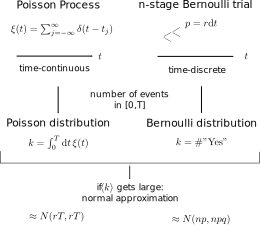
\includegraphics[width=0.9\linewidth]{Pics/overview_stochastic_processes}
	\caption{Relation between different stochastic processes and their corresponding distributions.}
	\label{fig:overviewstochasticprocesses}
\end{figure}





\chapter{Diffusion \& Random Walk}

\section{Random Walker}

The random walk can be used to model a variety of different phenomena just like
%
\begin{itemize}
	\item{the motion of a particle during diffusion}
	\item{the spread of mosquito infestation in a forest}
	\item{propagation of sound waves in a heterogeneous material}
	\item{money flow, stock prices}
\end{itemize}
%

%
\begin{theorem}[Model: Random Walker]
	%
	A random walker in $d$-dimensional space can be considered as a particle moving in steps of length $l$, while choosing each time a random, uncorrelated direction. Uncorrelated means that
	%
	\begin{equation}
	\expval{\vec{x}_n \cdot \vec{x}_m} = l^2 \delta_{nm}, \quad \vec{x}_n \in \R^d, n \in \Z
	\end{equation}
	%
	for averaging over the probability distribution of steps $\rho(\vec{x}_n)$.
	%
\end{theorem}
%

Thus, the displacement $\vec{x}$ of a random walker after $N$ steps is given by
%
\begin{equation}
\vec{x} = \sum^N_{n = 1}{\vec{x}_n} \quad \mathrm{with} \quad \expval{\vec{x}} = \vec{0}
\end{equation}
%
The mean square displacement $(\Delta \vec{x})^2$ equals the variance $\sigma^2$
%
\begin{align*}
\sigma^2 &= \expval{\vec{x}^2} - \expval{\vec{x}}^2 = \expval{\vec{x}^2} = (\Delta \vec{x})^2 \\ 
&= \expval{\left( \sum^N_{n = 1}{\vec{x}_n} \right)^2} = \sum^N_{n, m = 1}\expval{\vec{x}_n \cdot \vec{x}_m} = N l^2
\end{align*}
%
As we have $(\Delta \vec{x})^2 \sim N$ and $\Delta t \sim N $, the ratio $\frac{(\Delta \vec{x})^2}{\Delta t}$ is a constant in the continuum limit. This is quite unusual since a square term in the numerator appears.  

\section{Continuum Limit: Diffusion Equation}

We now consider the step sizes $|\Delta \vec{y}|$ of a random walker becoming infinitesimally small, with $p(\Delta \vec{y})$ being the probability for step $\Delta \vec{y}$:
%
\begin{gather}
\expval{\Delta \vec{y}_i} = \int{\dd[d]{\Delta y} \left[ \Delta y_i \, p(\Delta \vec{y}) \right]} = 0 \\
\expval{\Delta \vec{y}_i \, \Delta \vec{y}_j} = \int{\dd[d]{\Delta y} \left[ \Delta y_i \, \Delta y_j \, p(\Delta \vec{y}) \right]} = \expval{(\Delta \vec{y})^2} \frac{\delta_{ij}}{d}
\end{gather}
%
for $i, j = 1, 2, \, \dots, \, d$ vector components.

We can express the probability for a displacement of $\vec{x}$ after N steps $p_N(\vec{x})$ through the elementary relation
%
\begin{equation}
P_N(\vec{x}) = \int{\dd[d]{\Delta y} P_{N-1}(\vec{x} - \Delta \vec{y}) P(\Delta \vec{y})}
\end{equation}
%
Next, we perform a Taylor expansion of $P_N(\vec{x})$
%
\begin{align*}
P_N(\vec{x}) &\approx \int{\dd[d]{\Delta y} P(\Delta \vec{y}) \left[ 
	P_{N-1}(\vec{x}) - \Delta y_i \partial_i P_{N-1}(\vec{x}) + \frac{1}{2}  \Delta y_i \Delta y_j \partial_i \partial_j P_{N-1}(\vec{x}) \right]} \\
&= P_{N-1}(\vec{x}) + \frac{\expval{(\Delta \vec{y})^2}}{2 d} \nab^2 P_{N-1}(\vec{x})	
\end{align*}
%
We can define a continuum probability density $p(\vec{x},t)$ after the time $t = N \Delta t$
%
\begin{equation}
p(\vec{x},t) = p(\vec{x}, N \Delta t) := P_N(\vec{x})
\end{equation}
%
and now we can take the limit
%
\begin{equation}
\pdv{p}{t} = \lim_{\Delta t \to 0} \frac{P_N(\vec{x}) - P_{N-1}(\vec{x})}{\Delta t} = D \nab^2 p \quad \mathrm{with} \quad D = \frac{\expval{(\Delta \vec{y})^2}}{2 d \Delta t}
\end{equation}
%
This continuum limit exists if $D$ can be treated as a constant, i.e. if $\frac{\expval{(\Delta \vec{y})^2}}{\Delta t}$ is finite for $\Delta t \to 0$. The resulting equation is known as the diffusion equation.

\newpage
%
\begin{theorem}[Diffusion Equation]
	The \textit{diffusion equation} for a probability density $p(\vec{x}, t)$ reads
	%
	\begin{equation}
	\pdv{p(\vec{x}, t)}{t} = D \nabla^2 p(\vec{x}, t) \quad,
	\end{equation}
	%
	where $D$ is the diffusion coefficient with units $[D]=\mathrm{m}^2\,\mathrm{s}^{-1}$.
	Alternativly, we can start from the \textit{conservation equation}
	%
	\begin{equation}
	\pdv{p}{t} = - \nab \cdot \vec{J}
	\end{equation}
	with probability current $\vec{J}$, 
	which reads for the case of the diffusion equation $\vec{J} = -D \nab p$.
	%
\end{theorem}
%
Remark: The case of a position-dependent diffusion coefficient $D(\vec{x})$ is somewhat subtle, 
and requires some microscopic knowledge of the underlying system, see also the section on Ito and Stratonovich calculus.
% TODO: add text reference

\subsection*{Solving the diffusion equation}

The diffusion equation can be solved e.g. by doing a Fourier transformation of both sides
%
\begin{equation}
\pdv{p}{t} =  D \vec{k}^2 p
\end{equation}
%
leading to the k-space solution
%
\begin{equation}
p(\vec{k},t) = \F(p(\vec{x},t)) = \exp(-D \vec{k}^2 t)
\end{equation}
%
A Fourier transform backwards gives the fundamental solution (Green's function)
%
\begin{equation}
p(\vec{x},t) = \frac{1}{(4 \pi k t)^{d/2}} \exp(-\frac{\vec{x}^2}{4 k t})
\end{equation}
%
with the mean square spread $\sigma^2 \sim k t$, which is a spherically symmetric, multivariate normal distribution.

%
\begin{theorem}[Concept: Diffusion]
	%
	Diffusion is a net movement of particles from a region of high to a region of low concentration due to random motion of the single particles. 
	%
\end{theorem}
%

\newpage
\section{Random Force Model}

Another approach to diffusion is to consider a colloidal particle suspended in a fluid that is experiencing random forces $f(t)$ due to the interaction with the fluid molecules. 

Each fluid molecule is governed by the Hamiltonian equations of motion
%
\begin{equation}
	\dot{\vec{p}}_i = -\frac{\partial H}{\partial \vec{q}_i}, \quad 
	\dot{\vec{q}}_i = \frac{\partial H}{\partial \vec{p}_i}
\end{equation}
%
and their average velocity is characterized by the fluid's temperature $T$
%
\begin{equation}
	\frac{m}{2} \langle \vec{q}_i^{\,2} \rangle = \frac{k_B T}{2}
\end{equation}
%

\begin{remark}[Repetition: Equipartition Theorem]
	At thermal equilibrium, the system's energy, given by a Hamiltonian $H$, is distributed on its degrees of freedom $x_n$ via
	%
	\begin{equation}
		\expval{x_m \pdv{H}{x_n}} = \delta_{mn} k_B T
	\end{equation}
	%
	This holds for a microcanonical and canonical ensemble and relates temperature to the systems average energies.
\end{remark}

%
\begin{theorem}[Model: Random Forces]
	The motion of a particle under random forces $f(t)$ in one space dimension can be described by Newton's second law via
	%
	\begin{equation}
		m \ddot{x} + \gamma \dot{x} = f(t)
	\end{equation}
	%
	where $x(t)$ is the colloid's position and $\gamma$ is the damping constant.
	
	For long time scales $\tau_m >> \frac{m}{\gamma}$, inertia is negligible and we obtain the overdamped dynamics $\gamma \dot{x} = f(t)$. The random force is characterized through
	%
	\begin{itemize}
		\item{$\expval{f(t)} = 0$ (by symmetry)}
		\item{a vanishing correlation $\expval{f(t)f(t+\tau)} \to 0$ for $\tau \gg \tau_m$, with the correlation time $\tau_m$}
		\item{stationarity of the random forces: %
			\begin{equation}
				\frac{1}{\gamma^2}\int_{-\infty}^{\infty}{\dd{\tau} \expval{f(t)f(t+\tau)}} = 2D
			\end{equation}
			%
			with $[D] = \si{\meter \squared \per \second}$}
	\end{itemize}
	%
	In each case the average is taken over the probability distribution of the random force.
	%
\end{theorem}
%


\subsection*{Formal Solution}

A formal solution to the equation of motion without inertia reads
%
\begin{equation}
x(t) = x(0) + \frac{1}{\gamma} \int_0^t{\dd{t_1} f(t_1)}
\end{equation}
%

Defining $\Delta x := x(t) - x(0)$, we get by symmetry for the mean displacement
%
\begin{equation}
\expval{\Delta x(t)} = \frac{1}{\gamma} \int_0^t{\dd{t_1} \expval{f(t_1)}} = 0
\end{equation}
%
and for the mean square displacement
%
\begin{align*}
\expval{\Delta x^2} &= \frac{1}{\gamma^2} \expval{\left( \int_0^t{\dd{t_1} f(t_1)} \right) \left( \int_0^t{\dd{t_2} f(t_2)} \right)} \\
&= \frac{1}{\gamma^2} \int_0^t \dd{t_1} \int_0^t{\dd{t_2} \expval{f(t_1) f(t_2)}} \\
&= \frac{1}{\gamma^2} \int_0^t \dd{t_1} \int_{-t_1}^{t+t_1}{\dd{\tau} \expval{f(t_1) f(t_1 + \tau)}}\\
&= \frac{1}{\gamma^2} \int_0^t \dd{t_1} \int_{-\infty}^{\infty}{\dd{\tau} \expval{f(t_1) f(t_1 + \tau)}} + \O{D \tau_m}\\		
&= \frac{1}{\gamma^2} \int_0^t{\dd{t_1} \gamma^2 2 D} = 2 D t
\end{align*}
%

\subsection*{Calculating $D = D(T)$}

In order to calculate $D(T)$, we do a trick and add an elastic spring to the model
%
\begin{equation}
k x + \gamma \dot{x} = f(t)
\end{equation}
%
So at first we might ask what happens in reaction to a pulse response?
%
\begin{equation}
k x + \gamma \dot{x} = \rho_0 \delta(t) \quad \mathrm{with} \quad x(t) = 0 \, | \, t < 0
\end{equation}
%
The solution to this scenario is given by
%
\begin{equation}
x(t) = \rho_0 \chi(t), \quad \chi(t) = \frac{1}{\gamma} \exp(-\frac{t}{\sigma}) \Theta(t), \quad \sigma = \frac{\gamma}{k}
\end{equation}
%
We get back to the full problem, where the formal solutions reads
%
\begin{equation}
x(t) =  \int_0^{\infty}{\dd{\tau} f(t - \tau) \chi(\tau)}
\end{equation}
%
with $\expval{x(t)} = 0$ by symmetry and 

\begin{align*}
\expval{\Delta x^2} &= \frac{1}{\gamma^2} \expval{\left( \int_0^{\infty}{\dd{\tau_1} f(t-\tau_1) \chi(\tau_1)} \right) \left( \int_0^{\infty}{\dd{\tau_2} f(t-\tau_2) \chi(\tau_2)} \right)} \\
&= \int_0^{\infty} \dd{\tau_1} \int_0^{\infty} \dd{\tau_2} \expval{f(t-\tau_1) f(t-\tau_2)} \underbrace{\chi(\tau_1) \chi(\tau_2)}_{= \frac{1}{\gamma^2} \exp(- \frac{\tau_1 + \tau_2}{\sigma})} \\
&= \int_0^{\infty} \dd{\tau_1} \int_{-\tau_1}^{\infty} \dd{\tau} \expval{f(t-\tau_1) f(t-\tau_1 - \tau)}  \frac{1}{\gamma^2} \exp(- \frac{2\tau_1 + \tau}{\sigma}) \\
&= \int_0^{\infty} \dd{\tau_1} \int_{-\infty}^{\infty} \dd{\tau} \expval{f(t-\tau_1) f(t-\tau_1 - \tau)}  \frac{1}{\gamma^2} \exp(- \frac{2\tau_1 + \tau}{\sigma}) + \O{D\tau_m} \\
&= \frac{1}{\gamma^2} \int_0^{\infty} \dd{\tau_1} \exp(- \frac{2\tau_1}{\sigma}) \int_{-\infty}^{\infty} \dd{\tau} \expval{f(t-\tau_1) f(t-\tau_1 - \tau)} \underbrace{\exp(- \frac{\tau}{\sigma})}_{\approx 1, \, \tau_m \ll \sigma} \\
&= \frac{1}{\gamma^2} \frac{\sigma}{2} 2 D \gamma^2 = \frac{\gamma}{k}D
\end{align*}
%
At this point, we would like to make use of the equipartition theorem
%
\begin{equation}
\expval{\frac{k}{2}x^2} = \frac{k_B T}{2}
\end{equation}
%
As we have 
%
\begin{equation}
\expval{\frac{k}{2}x^2} = \frac{k}{2} \frac{\gamma}{k}D = \frac{k_B T}{2}
\end{equation}
%
we obtain the Stokes-Einstein-relation
%
\begin{equation}
D = \frac{k_B T}{\gamma}
\end{equation}
%


\subsection*{Numerical Solution: Explicit Euler Scheme}

Consider as a heuristic example a stochastic process where inertia is negligible 
%
\begin{equation}
	\gamma \dot{x} = f(t)
\end{equation}
%
A numerical solution for e.g. a particles position $x(t)$ depending on the random force $f(t)$ can be obtained from an explicit Euler scheme for discrete times $t_n = n \cdot dt$ and discrete positions $x_n = x(t_n)$. 

The updates 
%
\begin{equation}
	u_n = \int_{t_n}^{t_{n+1}} dt \frac{f(t)}{\gamma}
\end{equation}
%
have the properties
%
\begin{equation}
	\langle u_n \rangle = 0, \quad 
	\langle u^2_n \rangle = 2 D dt, \quad 
	\langle u_n u_{n+1} \rangle \approx 0
\end{equation}
%

The can be parameterized via $u_n \approx \sqrt{2D} dw_n$, where $dw_n \sim N(0,dt)$ are independent, normally distributed random variables. Finally, the explicit Euler scheme reads
%
\begin{equation}
	x_{n+1} = x_n + \sqrt{2D} dw_n
\end{equation}
%
One needs to be careful if $D = D(x)$.


\subsection*{Examples for Diffusion Processes}

% Bitte ergänzen/korrigieren, das ist im handschriftlichen Skript schwer zu lesen ;-)

The damping of a colloid with radius $r$ constant is given by $\gamma = 6 \pi \eta r$.

For $r = \SI{1}{\micro\meter}$ and the viscosity of water $\eta = \SI{E-3}{\pascal\second}$
this yields $\gamma = \SI{2E-8}{\newton \second \per \meter}$ and $D = \frac{k_B T}{\gamma} = \SI{2E-13}{\meter\squared \per \second}$

For a protein with $r = \SI{2}{\nano\meter}$ in water this yields $\gamma = \SI{4E-11}{\newton \second \per \meter}$ and $D = \frac{k_B T}{\gamma} = \SI{E-10}{\meter\squared \per \second}$




\chapter{Langevin Equation and Fokker-Planck Equation}

\section{Langevin equation}

Langevin theory describes non-equilibrium systems by postulating a stochastic process, thus adding a noise term to fundamental equations. In its original form, Langevin theory was used to describe Brownian motion, e.g. of a particle suspended in a fluid.

\begin{theorem}[Definition of the Langevin equation]
	%
	The Langevin equation is a stochastic differential equation for the particle velocity
	%
	\begin{equation}
	\dot{x} = \underbrace{f(x)}_{\mathrm{drift}} + \underbrace{\sqrt{2D} \, \xi(t)}_{\mathrm{random \, noise}}
	\label{langevin}
	\end{equation}
	%
	\begin{itemize}
		\item $\xi(t)$ represents Gaussian white noise 
		\item{$f(x)$ describes diffusion in an effective potential $U(x) = - \int_0^{x}{\dd{x'} f(x')}$}
	\end{itemize}
	%
\end{theorem}

\subsection*{Generalisation to $m$ variables}
%
\begin{equation}
\dot{x}_i =f_i(\vec x) + \sum_{j=1}^m g_{ij}(\vec x) \xi_j(t)
\end{equation}
%
with $i = 1, \dots, n$ and $\xi_j(t)$ being independent Gaussian white noise functions $\expval{\xi_j(t) \xi_l(t')} = \delta_{jl} \delta(t - t')$, $j, l = 1, \dots, m$.

\newpage
\underline{Example I: Double-well Potential}

\begin{figure}[H]
	\centering
	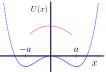
\includegraphics[width=0.7\linewidth]{Pics/doublewell_potential}
	\label{fig:doublewellpotential}
\end{figure}


$x(t = 0) = a$ \\

\underline{Example II: Escape over a Barrier}

\begin{figure}[H]
	\centering
	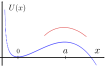
\includegraphics[width=0.7\linewidth]{Pics/escape_over_barrier}
	\label{fig:escapeoverbarrier}
\end{figure}

$x(t = 0) = 0$, escape rate? \\


\newpage
\subsection*{Numerics for the Langevin Equation}

\begin{theorem}[Euler Scheme]
	The Langevin equation $\dot{x} = f(x) + \sqrt{2D} \, \xi(t)$ leads, using the Euler scheme, to the following update-rule
	%
	\begin{equation}
	\hat{x}_{n+1} = \hat{x}_n + f(\hat{x}_n) \dd{t} + \sqrt{2 D \dd{t}} N_n
	\end{equation}
	%
	with $D = D_0$, $t_i = i \dd{t}$, $x_i = x(t_i)$ and the independent Gaussian variables $N_n \sim N(0,1)$. The numerical error scales as $|\hat{x}_n - x_n| \sim \O{\dd{t}^{3/2}}$.
\end{theorem}

N.B. $X_{n+1} - x_n = \sqrt{2D} dw$ with $\langle \mathrm{d}w^2 \rangle = 2D \mathrm{d}t$

Care needs to be taken if $D = D(x)$. 
% What follows in this case?


\section{Fokker-Planck-Equation}

\subsection*{Derivation of Fokker-Planck-Equation}

\begin{remark}[Repetition: Ordinary Diffusion]
	
	For the example of ordinary diffusion in one space dimension
	%
	\begin{equation}
	\dot{x} = \xi(t), \, x(0) = 0 \quad \mathrm{with} \quad \expval{x(t)} = 0, \, \expval{x^2(t)} = 2 D t
	\end{equation}
	%
	the probability density is given by
	%
	\begin{equation}
	p(x,t) = \frac{1}{\sqrt{2 \pi}} \frac{1}{\sqrt{2 D t}} \exp(-\frac{x^2}{4 D t})
	\end{equation}
	%
	fulfilling the Diffusion equation
	%
	\begin{equation}
	\pdv{p(x,t)}{t} = D \pdv[2]{p(x,t)}{x}
	\end{equation}
	%
\end{remark}

Considering the general case $\dot{x} = f(x) + \sqrt{2D} \, \xi(t)$, we would like to find an operator $\hat{L}$ such that
%
\begin{equation}
\pdv{p(x,t)}{t} = \hat{L} p(x,t)
\end{equation}
%
Therefore, we discretize time and take a look how a sub-ensemble of $p(x,t)$ at $x_n$ will evolve during a time step from $p(x,t_n)$ to $p(x,t_{n+1})$. For this we are using the Markov-Property: 
%
\begin{align*}
	p(x,t_{n+1}|x_0,t_0) &= \int{\dd{x}_n p(x,t_{n+1},x_n,t_n|x_0,t_0)} \\
	&= \int{\dd{x}_n p(x,t_{n+1}|x_n,t_n)} \, p(x_n,t_n|x_0,t_0) \\
	&= \int{\dd{x}_n N(x_n+f(x_n), 2D \dd{t}) p(x_n,t_n|x_0,t_0)}
\end{align*}
%
The left term captures the probability to have been at $x_n$ at $t = t_n$, the right term the probability to have moved from $x_n$ to $x_{n+1}$.

This is already an implicit solution in terms of a convolution of the probability density with a family of normal distributions, but it is of little practical use. 
%
\begin{remark}[A Remark about Units]
	Unlike probabilities, probability densities for positions have units of inverse length! Therefore we are integrating over a two-point probability density which has units of inverse length squared
	%
	\begin{align*}
		[p(x,t_{n+1}|x_0,t_0)] &= \si{\per \meter} \\
		[p(x,t_{n+1},x_n,t_n|x_0,t_0)] &= \si{\per \meter \squared}
	\end{align*}
	%	 
\end{remark}
%
So, let us define the following abbreviations in order to evaluate this convolution further 
%
\begin{align*}
	p(x,t_n) = \int \dd x_n I(x_n, y) |_{y = x-x_n} \quad &\mathrm{with} \quad I(x_n,y) = p(x_n) n(x_n,y), \\ 
	&\mathrm{and} \quad n(x_n,y) = N(f(x_n) \dd t, 2 D \dd t)
\end{align*}
%
The integrand $I(x,y)$ will contribute only for small $y = \O{\dd t}$, which means $x_n \approx x$, so we can Taylor expand $I(x_n,y)$ in $x_n$ around $x$:
%
\begin{equation}
I(x_n,y) = I(x,y) + \pdv{I(x_n,y)}{x_n} \big|_{x_n = x} (x_n-x) + \pdv[2]{I(x_n,y)}{x_n} \big|_{x_n = x} \frac{(x_n-x)^2}{2}
\end{equation}
%
Inserting this into the convolution integral leads to
%
\begin{align*}
	p(x,t_{n+1}) &= \int{\dd{y} I(x,y)|_{x_n = x-y}} \\
	&= \int\dd y \left( p(x) n(x,y) - \pdv{x} (p(x) \, n(x,y) \, y ) + \pdv[2]{x} (p(x) \, n(x,y) \, \frac{y^2}{2})\right) \\
	&= p(x) \int \dd{y} n(x,y) - \pdv{x} \left(p(x) \int \dd{y} n(x,y) \, y \right) + \pdv[2]{x} \left(p(x) \int \dd{y} n(x,y) \, \frac{y^2}{2} \right)
\end{align*}
%
The integrals that are occurring in this step are know as Kramers-Moyal coefficients:
%
\begin{align*}
	&\int \dd{y} n(x,y) = 1 \\
	&\int \dd{y} n(x,y) \, y = f(x) \dd{t} \\
	&\int \dd{y} n(x,y) \, \frac{y^2}{2} = D \dd{t} + \frac{1}{2}[f(x)]^2 \dd{t^2} = D \dd{t} + \O{\dd{t}^2}
\end{align*}
%
which give us
%
\begin{equation}
p(x,t_{n+1}) = p(x,t_n) - \pdv{x} [p(x,t_n) f(x) \dd{t}] + \pdv[2]{x}[p(x,t_n) D]\dd{t}
\end{equation}
%
and thus
%
\begin{equation}
\frac{p(x,t_{n+1}) - p(x,t_n)}{\dd{t}} =  -\pdv{x} [p(x,t_n) f(x)] + \pdv[2]{x}[p(x,t_n) D]
\end{equation}
%

Taking the time step to zero, we have finally derived the Fokker-Planck equation.
%
\begin{theorem}[Fokker-Planck equation]
	The Fokker-Planck equation is a partial differential equation for a probability density $p(x)$, which reads for an ensemble governed by the Langevin equation (\ref{langevin}) as follows
	%
	\begin{equation}
	\pdv{t} p(x,t) = -\pdv{x}[p(x,t) \, f] + D \pdv[2]{x} p(x,t)
	\end{equation}
	%
\end{theorem}
%
The structure of the Fokker-Planck equation is similar to the Schrödinger equation, i.e. solution methods from QM can be borrowed (take a look at the Risken book \cite{Risken1996}). 

\subsection*{Application to Diffusion in a Potential}

We consider diffusion in a potential $U(x)$ (now we care about physical units!)
%
\begin{equation}
\dot{x} = - \frac{1}{\gamma} \pdv{U}{x} + \xi
\end{equation}
%
and ask for the steady state $\pdv{t} p(x,t) = 0$. Hence, the Fokker-Planck equation reads
%
\begin{align*}
	0 &= \nab [(\frac{1}{\gamma} \nab U) p] + D \nab^2 p 
	= \nab [\frac{1}{\gamma} \nab U p + D \nab p] \\
	\Rightarrow c &= \frac{1}{\gamma} \nab U p + D \nab p
\end{align*}
%
thus, if $c = 0$, we get
%
\begin{equation}
\pdv{x} \ln p = \frac{\nab p}{p} = - \frac{1}{\gamma} \frac{\nab U}{p}
\end{equation}
%
and 
%
\begin{equation}
p \sim \exp(-\frac{U}{\gamma D}) = \exp(-\frac{U}{k_B T})
\end{equation}
%
with $D = \frac{k_B T}{\gamma}$, i.e. we recover the Boltzmann distribution. If $c$ would not be zero, the solution could not be normalized. Another explanation, why $c = 0$, is based on the Fokker-Planck-equation being interpreted as conservation equation 
%
\begin{equation}
\dot{p} = - \nab \vec{J} \quad \mathrm{with} \quad \vec{J} = \frac{1}{\gamma} \nab U p + D \nab p
\end{equation}
%
of the current $\vec{J}$. At equilibrium, the current must vanish and thus we have
%
\begin{equation}
\lim_{t \to \infty} \vec{J} = c = 0
\end{equation}
%


\subsection*{Eigenvalue Spectrum of $\hat{L}$}

The probability density can be expressed in terms of eigenfunctions of the Fokker-Planck operator $\hat{L}$ with $\dot{p} = \hat{L} p$
%
\begin{equation}
\hat{L} \phi_n(x) = \lambda_n \phi_n(x)
\end{equation}
%
through
%
\begin{equation}
p(x,t) = \sum a_n \phi_n(x) \exp(\lambda_n t)
\end{equation}
%
If $\lambda_0 = 0$, then the corresponding eigenfunction is a steady state $\phi_0$. The slowest decaying mode determines hopping rates and it is $0 \leq \lambda_1 \leq \lambda_2 \dots$. 

\begin{comment}
This can be shown the following way:
%
\begin{equation}
	1 = \int \mathrm{d}x p(x,t) = \sum_n a_n \exp{\lambda_n t} \int \mathrm{d}x \phi_n(x) 
\end{equation}
%
If $\lambda_n \neq 0$, then $\int  \mathrm{d}x \phi_n(x)  = 0$ and $\exists x: \phi_n(x) = 0 $ % why?

So $0 \geq p(x,t)$ and thus $\Re(\lambda_n) \leq 0$
\end{comment}

But why are the $\lambda_n$ real? We have $\hat{L} \neq \hat{L}^*$, which means $\hat{L}$ is not Hermitian.
%
\begin{equation}
\expval{\hat{L}g,h}= \int \dd{x} (\hat{L}g)h = \int \dd{x} g \hat{L}^*h = \expval{g,\hat{L}^* h} \quad \forall g(x), h(x)
\end{equation}
%
By partial integration we see that the adjoint operator has the form
%
\begin{equation}
\hat{L}^*h = f \pdv{h}{x} + D \pdv[2]{h}{x}
\end{equation}
%
If $f(x) = - \pdv{U(x)}{x}$, we can define a Hermitian operator by
%
\begin{equation}
A = T^{-1} L T \quad \mathrm{with} \quad T = \exp(+\frac{\beta U}{2}), \, \beta = \frac{1}{D}
\end{equation}
%
The operator is self-adjoint $\hat{A} = \hat{A}^*$ and thus all eigenvalues are real. $\hat{A}$ and $\hat{L}$ have the same eigenvalues. 

\begin{theorem}[Backward Fokker-Planck Equation]
	$p = p(x_1,t|x_0,0) = p(x_1,0|x_0,-t)$, which gives the backward Fokker-Planck equation
	%
	\begin{equation}
	\dot{p} = \hat{L}_{x_1} p = \hat{L}^*_{x_0} p = \left[ + f(x) \pdv{x_0} + D \pdv[2]{x_0} \right] p(x_1,0 \, | \, x_0,-t)
	\end{equation}
	%
\end{theorem}

\subsection*{Boundary Conditions Matter}

\underline{1) Reflecting Boundary Conditions (No-Flux / Robin B.C.)}

The probability current $\dot{p} = -J$ vanishes
%
\begin{equation}
J(x_1) = J(x_2) = 0
\end{equation}
%
and
%
\begin{equation}
\int_{x_1}^{x_2} \dd{x} p(x,t) = 1 \rightarrow
\frac{\mathrm{d}}{\mathrm{d}t} \int_{x_1}^{x_2} \dd{x} p(x,t) = 0
\end{equation}
%
In this case the steady-state distribution $p^*(x) = \phi_0(x)$ exists. Similar results hold for a confinement potential $\lim_{x \to x_1, x_2} U(x) \to \infty$. \\

\underline{2) Absorbing Boundary Conditions}

For absorbing boundary conditions we impose $p(x_2,t) = 0$ (Dirichlet boundary conditions). Therefore
%
\begin{equation}
0 > \dv{t} \int \dd{x} p(x,t) = \int \dd{x} \dv{p(x,t)}{t} = \int_{-\infty}^{x_2} -\pdv{J}{x} = -J(x_2)
\end{equation}
%
is the flux to the absorber. 

No steady-state solution exists (non-trivial / normalizable to one) and all eigenvalues are strictly negative. $\lambda_1 < 0$ sets the slowest time scale.

In the limit of long times $t \to \frac{1}{\lambda_1}$, the porbability density can be decomposed into $p(x,t) = a(t) p_1(x)$ with $a(t) \sim \exp(-\lambda_1 t)$. 

\begin{remark}[Boundary Conditions and Functional Analysis]
	Changing the boundary conditions changes also the eigenvalues and the adjoint operator (boundary terms might pop up) and thus you will get each time a different operator in terms of functional analysis. 
\end{remark}


\section{Master Equation}

The master equation (M-equation) describes time-continuous, continuous state variables and it is of the general form
%
\begin{equation}
	\frac{\partial}{\partial t} P(x,t) = \int \mathrm{d}x_1 \underbrace{w(x|x_1) P(x_1,t)}_{= \mathrm{gain}} - \underbrace{w(x_1|x) P(x,t)}_{= \mathrm{loss}}
\end{equation}
%


$w(x|x_1)$ is the transition rate density for the process $x_1 \to x_2$, i.e. $w(x|x_1) \Delta x_1 \Delta x_2 \Delta t$ is the probability of a transition from $[x_1, x_1 + \Delta x_1]$ to $[x_2, x_2 + \Delta x_2]$ in the time interval $\Delta t$

The Fokker-Planck equation is a special case of the master equation. 

For a time-continuous, discrete state variable the master equation reads 
%
\begin{equation}
	\frac{\mathrm{d}}{\mathrm{d}t} P_n(t) = \sum_m w_{nm} p_m(t) - w_{mn} p_n(t)
\end{equation}
%
where $w_{nm}$ is the transition rate $m \to n$. 


\subsection*{Example I: Fermi's Golden Rule}

Let $\hat{H} = \hat{H}_0 + \varepsilon \hat{H}_1 \Theta(t)$ be a perturbed Hamiltonian and $| m_0 \langle$ be an eigenstate of the unperturbed Hamiltonian $\hat{H}_0$ and the initial state.

The transition rate $m_0 \to n$ is given by Fermi's Golden rule
%
\begin{equation}
	w_{nm_0} = \frac{2\pi}{\hbar} \varepsilon^2 |\langle n | \hat{H}_1 | \rangle| \rho + \mathbb{O}(\varepsilon^4)
\end{equation}
%

\subsection*{Example II: Radioactive Decay}

Let $n$ be the number of particles that is left (i.e. not decayed). 
%
\begin{equation}
	T_{\delta t}(n|m) = 
	\begin{cases} 
		0 								&\quad n > m \\
		m \gamma \delta t 	&\quad n = m \\
		\mathbb{O}(\delta t^2) &\quad n < m
	\end{cases}
\end{equation}
%

% What is m? 

The master equation reads 
%
\begin{equation}
	\frac{\mathrm{d}}{\mathrm{d}t} p_n = \gamma(n+1) p_{n+1} - \gamma(n) p_n
\end{equation}
%
where $N = \langle n \rangle = \sum_n p_n$ and
%
\begin{equation}
	\frac{\mathrm{d}}{\mathrm{d}t} N = - \gamma(n) N
\end{equation}
%
and thus $N = N_0 \exp(-\gamma t)$.



\chapter{Dynkin Equation}

\section{Mean First Passage Times and Dynkin Equation}

We consider diffusion in some potential landscape $\gamma \dot{x} = - \pdv{U}{x} + \xi(t)$ with initial conditions $p(x,0) = \delta(x-x_1)$ and absorbing boundary conditions $p(x_2,t) = 0$, i.e, $\dot{p} = -\nabla J$ where $J(x_2,t)$ is the current to the absorbing boundary conditions.

\begin{theorem}[Mean First Passage Time (MFPT)]
	%
	\begin{equation}
	\tau(x_2|x_1) = \int_0^{\infty} \dd{t} t J(x_2,t|x_1,0)
	\end{equation}
	%
\end{theorem}

Our goal is to derive an equation for $\tau$ in the process 
%
\begin{equation}
	x_1 \underbrace{\longrightarrow}_{\Delta t} x^\prime \underbrace{\longrightarrow}_{\tau(x_2| x^\prime)} x_2
\end{equation}
%
If $\Delta t$ is small and kept constant (and we ask which positions can we reach within $\Delta t$) we have
%
\begin{equation}
	\tau(x_2|x_1) = \Delta t + \int_{-\infty}^{x_2} \dd{x'} \tau(x_2|x') p(x',\Delta t|x_1,0)
\end{equation}
%
and we take the derivative with respect to $\Delta t$
%
\begin{equation}
	\frac{\mathrm{d} \tau(x_2|x_1)}{\mathrm{d \Delta t}} = 
	0 = 1 + \int_{-\infty}^{x_2} \dd{x'} \tau(x_2|x') \hat{L}_{x'} p = 1 + \int_{-\infty}^{x_2} \dd{x'} \hat{L}^*_{x'} \tau(x_2|x') p
\end{equation}
%
so, if $\Delta t \to 0$ then $p(x',\Delta t|x_1,0) \to \delta(x-x_1)$,
and we get the \textit{Dynkin equation}
%
\begin{equation}
-1 = \hat{L}^*_{x_1} \tau(x_2|x_1)
\end{equation}
%

\subsection*{Application to Diffusion}

Let consider once again the example of diffusion
%
\begin{equation}
\gamma \dot{x} = - \pdv{U}{x} + \xi(t) \quad \expval{\xi(t)\xi(t')} = 2D \delta(t-t')
\end{equation}
%
with the initial condition $p(x,0) = \delta(x-x_1)$ and boundary conditions $p(x_2,t) = 0$. Let $v = \pdv{x_1} \tau(x_2 | x_1)$, so the Dynkin equation reads
%
\begin{equation}
-1 = D v' - \frac{U'}{\gamma}v
\end{equation}
%
which we multiply by $\frac{1}{D}\exp(-\beta U)$
%
\begin{equation}
-\frac{1}{D}\exp(-\beta U) = v'\exp(-\beta U) - \beta v \exp(-\beta U) = \dv{x_1}[v \exp(-\beta U)]
\end{equation}
%
to get
%
\begin{equation}
v = -\frac{1}{D}\exp(-\beta U) \left[ \int_{-\infty}^{x_1} \dd{x'} \exp(-\beta U) + c \right]
\end{equation}
%
If we assume $\lim_{x\to -\infty} U(x) = +\infty$, then $|v| < \infty$ and $c = 0$. With one more integration we get
%
\begin{equation}
\tau(x_2,x_1) = \frac{1}{D} \int_{x_1}^{x_2} \exp(\beta U(x')) \left[ \int_{-\infty}^{x'} \dd{x''} \exp(-\beta U(x'')) \right]
\end{equation}
%
Note that the integration constant of the second integration must be zero due to $\tau(x_2 | x_2) = 0$

\section{Kramers Escape Rate Theory}

We consider the escape of particles over an energy barrier $\Delta E$ and assume $\beta \Delta E \gg 1$ to calculate $\tau(x_2|x_1)$. $\int \dd{x''}$ is sizeable only nearby $x_a$, $\int \dd{x'}$ is sizeable only nearby $x_b$. We do a standard trick: quadratic expansion around $x_a$ and $x_b$
%
\begin{equation}
U(x'') = U(x_a) + \frac{1}{2} U''(x_a) (x''-x_a)^2 + \dots
\end{equation}
%
with $U''(x_a) = k_a = \gamma/\tau_a$, which introduces a time-scale. Similarly
%
\begin{equation}
U(x') = U(x_b) + \frac{1}{2} U''(x_b) (x'-x_b)^2 + \dots
\end{equation}
%
with $U''(x_b) = -k_b = -\gamma/\tau_b$. So lets evaluate our integrals
%
\begin{align*}
	\int_{-\infty}^{x'} \dd{x''} \exp(-  \frac{1}{2} \beta U''(x_a) (x''-x_a)^2)
	&\approx \int_{-\infty}^{\infty} \dd{x''} \exp(-  \frac{1}{2} \beta U''(x_a) (x'-x_a)^2) \\ 
	&= \sqrt{2 \pi \sigma^2}
\end{align*}
%
with $\sigma^2 = \frac{\tau_a}{\beta \gamma}$ and
%
\begin{align*}
	\int_{-\infty}^{x'} \dd{x''} \exp(+\frac{1}{2} \beta U''(x_b) (x'-x_b)^2)
	&\approx \int_{-\infty}^{\infty} \dd{x''} \exp(+\frac{1}{2} \beta U''(x_b) (x'-x_b)^2) \\ &= \sqrt{2 \pi \frac{\tau_b}{\beta \gamma}}
\end{align*}
%
so
%
\begin{equation}
\tau(x_2 | x_1) = \frac{1}{D} \frac{2 \pi \sqrt{\tau_a \tau_b}}{\beta \gamma} \exp(\beta \Delta E) = 2 \pi \sqrt{\tau_a \tau_b} \exp(\beta \Delta E)
\end{equation}
%
\begin{theorem}[Kramers escape rate]
	%
	\begin{equation}
	r = \frac{1}{\tau(x_2 | x_1)} \sim \underbrace{\exp(-\beta \Delta E)}_{\mathrm{Arrhenius factor}}
	\end{equation}
	%
\end{theorem}
%

\section{Diffusion to Capture}

As an example, we consider a diffusing particle released at position $x_0$ between two absorbing plates at positions $x_1$ and $x_2$. 

The question is: What is the probability of getting absorbed at either of the two plates?
%
\begin{align*}
P(x, t=0) = \delta(x-x_0) \\
P(x_1, t) = P(x_2, t) = 0
\end{align*}
%
The probability of becoming absorbed at $x = x_1$ when starting at $x_0$ reads $\pi_1(x_0)$. We have $\pi_1(x_1) = 1$ and $\pi_1(x_2) = 0$.


\subsection*{Solution 1}

We will now consider a time step $\Delta t$ as we did for the derivation of the Dynkin equation in order to find an explicit expression for $\pi_1(x_0)$:
%
\begin{equation*}
\pi_1(x_0) = \int_{x_1}^{x_2} \dd{x} \pi_1(x) P(x, \Delta t | x_0, 0) 
= \int_{0}^{\infty} \dd{t} J(x_1,t | x_0,0)
\end{equation*}
%
Now we take the partial derivative with respect to $\Delta t$ 
%
\begin{equation*}
0 = \int_{x_1}^{x_2} \dd{x} \pi_1(x) \underbrace{\pdv{\Delta t} P(x, \Delta t | x_0, 0)}_{\hat{L} P}
\end{equation*}
%
and perform partial integration
%
\begin{equation*}
0 = \int_{x_1}^{x_2} \dd{x} \hat{L}^* \pi_1(x) \underbrace{P(x, \Delta t | x_0, 0)}_{\to \, \delta(x-x_0) \, \mathrm{for} \, \Delta t \to 0}
\end{equation*}
%
so we obtain
%
\begin{equation*}
0 = \hat{L}^* \pi_1(x)
\end{equation*}
%
Thus, $\pi_1(x_0)$ must be a linear function and taking the boundary conditions into account we conclude $\pi_1(x_0) = \frac{x_2-x_0}{x_2-x_1}$.


\subsection*{Solution 2}

Another way to compute this is the method of images. So 
%
\begin{equation}
P(x,t) = N(x_0, 2Dt) - N(2x_1-x_0, 2Dt) - N(2x_2 - x_0, 2Dt)
\end{equation}
%
and $\pi_1$ could be calculated directly. (Stream of anti-particles is released and annihilates particles at the boundary).

\section{Polya's theorem}

We consider diffusion in $\R^d$ to a d-dimensional absorbing ball. We ask for the probability $p(R_0)$ for a particle initially released at distance $R_0$ to hit the target ball. For $d = 1$ and $d = 2$ we have $p(R_0) = 1$, but for $d = 3$ $p(R_0) = \frac{R_1}{R_0}$

Note that for $d = 3$, the characteristic arrival time must scale with $\sqrt{R^2_0/D}$ with a power-law tail $\sim t^{-3/2} \exp(- (R_0-R_1)^2/4 D t)$ and the mean first passage time diverges.

\begin{comment}
% This parts need to be connected to the previous part

Infinite reservoir: 
%
\begin{equation}
0 \overset{!}{=} \dot{c} = D \nabla^2 c
\end{equation}
%
so $c(\vec{x}) = c_0$ for $|\vec{x}| \to \infty$ and $c(\vec{x}) = 0$ for $\vec{x} \in S$ where $S$ is the absorbing surface

For diffusion to an absorbing sphere of radius $a$ it is $J = 4 \pi D a c_0$. 

The diffusion equation is formally equivalent to the Poisson equation of the electrostatic potential. 

Diffusion to a disk-like absorber auf diameter $2 s$: $J = 4 D s c_0$. 
\end{comment}


\chapter{Synchronisation}

\section{Active Oscillators}

An active oscillator is a non-conservative oscillator, e.g. energy is lost through damping. An example is the 
%
\begin{theorem}[Van-der-Pol oscillator]
	%
	\begin{equation}
	m \ddot{x} - \gamma (\frac{1}{4} \Lambda - x^2) \dot{x} + kx = 0
	\label{van_der_pol_oscillator}
	\end{equation}
	%
\end{theorem}
%
The Van-der-Pol oscillator undergoes a so-called Hopf bifurcation as a function of parameter $\Lambda$: For $\Lambda < 0$ $x = 0$ is stable and for $\Lambda > 0$ limit-cycle oscillations occur. Equation (\ref{van_der_pol_oscillator}) can be transformed into Hopf normal form. 

Other examples are the 
%
\begin{theorem}[Hopf oscillator]
	%
	An active oscillator with non-linear damping of the form
	%
	\begin{equation}
	\dot{z} = i \omega_0 z + \mu(\Lambda - |z|^2)z \quad \mathrm{with} \quad z \in \C
	\end{equation}
	% 
	It is used e.g. to describe the limit cycle of electric circuits involving a vacuum tube or in biology to model the activation potential of neurons.
\end{theorem}
%
and a phase oscillator with $\dot{\varphi} = \omega_0$. 

\subsection*{Hopf normal form of Van-der-Pol oscillator}

We set $y = \dot{x}$, $\omega = \sqrt{k/m}$. The idea is to introduce $z \approx x - \frac{i}{\omega} y$, so we do the ansatz (in order to avoid quartic terms / the method is called Center Manifold technique)
%
\begin{align*}
	z &= \sum_{k}^{\infty}\sum_{l}^{\infty}{d_{k,l}x^l y^{k-l}} \\
	&= x - \frac{i}{\omega} y + d_{10}y + d_{33}x^3 + d_32 x^2 y + d_{31} xy^2 + d_{30} y^3 + \dots
\end{align*}
%
The back transformation is given by
%
\begin{align*}
	x &= \frac{z + \bar{z}}{2} + e_1 z^3 + e_2 z^2 \bar{z} + e_3 z \bar{z}^2 + e_4 \bar{z}^3 \dots \\
	y &= i \omega \frac{z - \bar{z}}{2} + f_1 z^3 + f_2 z^2 \bar{z} \dots
\end{align*}
%
so that
%
\begin{equation}
\dot{z} = h(z, \bar{z}) = Fz + G z^2 \bar{z} + \mathrm{h.o.t.}
\end{equation}
%
and for appropriate $d_{k,l}$ we have i) no quadratic terms, ii) no term in $\bar{z}$ and iii) no terms proportional to $z^3, z\bar{z}^2, \bar{z}^3$. We find that

%
\begin{align*}
	F &= i \omega_0 + \frac{\gamma}{8m} \Lambda + \O{\Lambda^2} \\
	G &= \frac{\gamma}{8m} + \O{\Lambda}
\end{align*}
%
and we get
%
\begin{equation}
\dot{z} = i (\omega_c - \omega_1 |z|^2)z + \mu(\Lambda - |z|^2)
\end{equation}
%
with $\omega_c = \omega_0$, $\omega_1 = \O{\Lambda}$ and $\mu = \frac{\gamma}{8m}$

\section{Hopf-oscillator with noise}

We now add a noise term to the Hopf-oscillator
%
\begin{equation}
\dot{z} = i \omega_0 z + \mu(\Lambda - |z|^2)z + (i \xi_{\varphi} + \xi_A) z
\end{equation}
%
with 
%
\begin{equation*}
	\expval{\xi_{\varphi}(t)\xi_{\varphi}(t')} = 2 D_{\varphi} \delta(t-t') \quad \expval{\xi_A(t)\xi_A(t')} = 2 D_A \delta(t-t') \quad
	\expval{\xi_{\varphi}(t)\xi_A(t')} = 0
\end{equation*}
%
and map $z$ on a phase $\varphi$ and amplitude $A$ via $z = A e^{i \varphi}$ so that
%
\begin{equation}
\left( \frac{\dot{A}}{A} + i \dot{\varphi} \right) z = \dot{z} = \dots
\end{equation}
%
and
%
\begin{equation}
\frac{\dot{A}}{A} + i \dot{\varphi} = i \omega_0 + \mu(A_0^2- A^2) + i \xi_{\varphi} + \xi_A
\end{equation}
%
Assuming $\Lambda > 0$ and $\Lambda = A_0^2$, we get a noisy phase oscillator
%
\begin{equation}
\dot{\varphi} = \omega_0 + \xi_{\varphi}
\end{equation}
%
and an Ornstein-Uhlenbeck process for the amplitude
%
%
\begin{equation}
%
\begin{gathered}
A = A_0 + a \\
\dot{a} = \mu(A_0 + a)(-2 a A_0 + a^2) + \xi_A = -2\mu A_0 a + \xi_A + \O{a^2}
\end{gathered}
%
\end{equation}
%
with the properties
%
\begin{equation*}
	\expval{a(t)} = 0 \quad \expval{a(t)a(t')} = D_A \tau \exp{- \frac{|t-t'|}{\tau}} \quad \tau = \frac{1}{2 \mu A_0}
\end{equation*}
%
\begin{remark}[Remark]
	If we consider an ensemble average, the amplitude fluctuations will decay with $\tau$: 
	%
	\begin{equation*}
		\bar{a}(t) = \expval{a(t)} \quad \mathrm{with} \quad \dv{d} \bar{a} = - \frac{\bar{a}}{\tau}
	\end{equation*}
	%
\end{remark}

\subsection*{Manifestation of Phase Noise}

We can characterize noisy oscillations in terms of a phase correlation function
%
\begin{equation}
C(t) = \expval{\exp(i \varphi(t_0)) \exp(-i \varphi(t_0 + t))}
\end{equation}
%
with $|C(t) = \exp(-D_{\varphi} t)|$, so
%
\begin{equation*}
	\frac{z(t_0)}{A_0} \frac{\bar{z}}{A_0} \approx \exp(\varphi(t_0)-\varphi(t_0+t)) \to \exp(i \omega_0 t) \quad \mathrm{if} \quad D_{\varphi} = 0
\end{equation*}
%
And we can have a look at the power spectral density 
%
\begin{equation}
S_y(\omega) = |\tilde{y}(\omega)|^2
\end{equation}
%
with $y = \exp(i \varphi)$ and its Fourier transform $\tilde{y}(\omega)$. 

\subsection*{Two coupled oscillators}

Two phase oscillators are coupled by the coupling $c$ leading to the ODE system
%
\begin{equation}
%
\begin{gathered}
\dot{\varphi}_L = \omega_L + c(\varphi_L - \varphi_R) \\
\dot{\varphi}_R = \omega_R + c(\varphi_R - \varphi_L)
\end{gathered}
%
\end{equation}
%
We introduce a phase difference of $\delta = \varphi_L - \varphi_R$
%
\begin{equation}
\dot{\delta} = \Delta \omega + c(\delta) - c(-\delta)
\end{equation}
%
with frequency mismatch $\Delta \omega = \omega_L - \omega_R$. A Fourier expansion of the coupling function yields 
%
\begin{equation}
c(\delta) = c(\delta + 2 \pi) = \sum_n{C_n' \cos(n \delta) + C_n'' \sin(n \delta)}
\end{equation}
%
Only the odd coupling terms contribute to synchronization, often $c(\delta)$ is dominated by the first Fourier mode and we end up at the Adler equation ($\lambda = - 2 c_1''$)
%
\begin{equation}
\dot{\delta} = \Delta \omega - \lambda \sin(\delta)
\end{equation}
%
If $|\Delta \omega| < |\lambda|$, we have fixed points for $\delta^* = \sin^{-1} \left( \frac{\Delta \omega}{\lambda} \right)$. The stability of the fixed points is determined by $\gamma \dot{\delta} = - \pdv{U}{\delta}$ and the effective potential $U = -\gamma \Delta \omega \delta - \gamma \lambda \cos(\delta)$. 

Images missing!

% Mapping synchronization to diffusion

\subsection*{Synchronization in the Presence of Noise}

If we consider two coupled phase oscillators with noise
%
\begin{gather}
	\dot{\varphi}_1 = \omega_1 - \frac{\lambda}{2} \sin(\varphi_1 - \varphi_2) + \xi_1(t) \\
	\dot{\varphi}_2 = \omega_2 - \frac{\lambda}{2} \sin(\varphi_2 - \varphi_1) + \xi_2(t)
\end{gather}
%
we obtain the noises Adler equation for the phase difference $\delta = \varphi_1 - \varphi_2$
%
\begin{equation}
\dot{\delta} = \Delta \omega - \lambda \sin(\delta) + \xi
\end{equation}
%
Here, and Gaussian white noise $\xi(t)$ represents Gaussian white noise with $\expval{\xi(t)\xi(t')} = 2 (D_L + D_R) \delta(t-t')$.

\begin{remark}[Remark: How to add two noise terms ]
	%
	\begin{equation*}
		\xi(t) = \xi_L(t) - \xi_R(t)
	\end{equation*}
	%
	with $\expval{\xi(t)} = 0$ and 
	%
	\begin{align*}
		\expval{\xi(t)\xi(t')} &= \expval{\xi_L(t)\xi_L(t')} + \expval{\xi_R(t)\xi_R(t')} + \expval{\xi_L(t)\xi_R(t')} \\
		&= 2D_L \delta(t-t') + 2D_R \delta(t-t') + 0 \\
		&= 2 (D_L + D_R) \delta(t-t')
	\end{align*}
	%	
\end{remark}
%
We can reinterpret the noisy Adler equation as the overdamped dynamics of a diffusing particle in a potential $U(x)$
%
\begin{equation}
\gamma \dot{\delta} = - \pdv{U}{\delta} + \xi
\end{equation}
%
and $U/\gamma = - \Delta \omega \delta - \lambda \cos(\delta)$. So what is the effect of noise? The steady state probability density reads
%
\begin{equation}
p^*(\delta) \sim \exp \left( -\frac{U(\delta)}{k_B T_{\mathrm{eff}}} \right) = \frac{1}{2 \pi I_0(ND)} \exp \left( -\frac{\lambda}{D} \cos(\delta) \right)
\end{equation}
%
with $D = k_B T_{\mathrm{eff}} \gamma$ and $\Delta \omega = 0$. So the first effect of noise is, that steady states are smeared out. The second effect are phase slips that occur
%
\begin{eqnarray*}
	\delta \approx 0 \longrightarrow \delta \approx 2 \pi \quad & \mathrm{with \; rate} \; G_+ \\
	\delta \approx 0 \longrightarrow \delta \approx -2 \pi \quad & \mathrm{with \; rate} \; G_-
\end{eqnarray*}
%
We can compute $G_{\pm}$ using Kramers escape rate theory
%
\begin{gather*}
	\frac{\gamma}{\tau_a} = U''|_{\delta = \delta_a} \Rightarrow \tau_a = \frac{1}{\sqrt{\lambda^2 - \Delta \omega^2}} \\ \\
	\frac{\gamma}{\tau_b} = U''|_{\delta = \delta_b} \Rightarrow \tau_b = \tau_a
\end{gather*}
%
and so
%
\begin{equation}
	G_+ = 2 \pi \tau_a \exp \left( \frac{- \Delta E}{D/\gamma} \right)
\end{equation}
%
The calculation for $G_-$ can be done analogously
%
\begin{equation}
	\frac{G_+}{G_-} = \exp(+ 2 \pi \Delta \omega / D)
\end{equation}
%
For $\Delta \omega = 0$ we get
%
\begin{equation}
	G_+ = G_- = \frac{\lambda}{2 \pi} \exp \left( - \frac{2 \lambda}{D} \right)
\end{equation}
%
The theory can be also extended to more than two oscillators.

\chapter{It$\bar{\mathrm{o}}$ versus Stratonovich Calculus}

If we are given an ODE, e.g. $\dot{x} = f(x)$, what does this mean? To answer this question, we are going to take a constructive approach and interpret the ODE as a rule to construct the solution. So we estimate the values $x_i = x(i \dd{t})$ and then take the limit $\dd{t} \to 0$.

\section{Numerical Motivation}

\subsection*{Deterministic ODE} 

For a deterministic ODE, we have various options to chose a scheme in order to solve them numerically. One could use either an explicit scheme like the Euler scheme 
%
\begin{equation}
	x_i = x_{i-1} + f(x_{i-1}) \dd{t}
\end{equation}
%
and implicit scheme 
%
\begin{equation}
	x_i = x_{i-1} + f(x_i) \dd{t}
\end{equation}
%
or a mixed scheme
%
\begin{equation}
	x_i = x_{i-1} + \frac{1}{2} [f(x_{i-1}) + f(x_i)]
\end{equation}
%
and all schemes will converge to the same limit.

\subsection*{Stochastic Differential Equations} 

Also for stochastic differential equations, such as $\dot{x} = f(x) + \sqrt{2 D(x)} \xi$, we may chose either an explicit scheme (It$\bar{\mathrm{o}}$) 
%
\begin{equation}
x_i = x_{i-1} + f(x_{i-1}) \dd{t} + \sqrt{2 D(x_{i-1})} N_i \sqrt{\dd{t}}
\end{equation}
%
with $N_i \in N(0,1)$. Alternatively, we could consider a mixed scheme (Stratonovich)
%
\begin{equation}
x_i = x_{i-1} + \frac{1}{2} [f(x_{i-1}) + f(x_i)] \dd{t} + \frac{1}{2} [\sqrt{2 D(x_{i-1})} + \sqrt{2 D(x_i)}] N_i \sqrt{\dd{t}}
\end{equation}
%
It is important to note that this time both schemes are different. (A purely implicit scheme for SDE is not discussed, because such schemes are rarely used in practice.) We can see this by doing the expansion
%
\begin{equation}
x_i = x_{i-1} + f(x_{i-1}) \dd{t} + \O{\dd{t}^{3/2}} + g(x_{i-1}) N_i \sqrt{\dd{t}} + g'(x_{i-1}) g(x_{i-1}) N_i^2 \dd{t}
\end{equation}
%
with $\expval{N_i^2} = 1$, so that the last term can not be neglected!

\section{Different Interpretations}

Having a look at the chain rule, one can see that the It$\bar{\mathrm{o}}$ and Stratonovich interpretation are indeed two different sorts of calculus. In Stratonovich interpretation the ordinary chain rule holds
%
\begin{equation}
\mathrm{(S)} \quad y = y(x), \quad \dot{y} = \pdv{y}{x} \dot{x}
\end{equation}
%
By contrast, in It$\bar{\mathrm{o}}$ interpretation we have $\dot{x}_k = f_k + g_{kl} \xi_l$ with $\expval{\xi_k(t) \xi_l(t')} = \delta_{kl} \delta(t-t')$ and the It$\bar{\mathrm{o}}$ chain rule applies
%
\begin{equation}
\mathrm{(I)} \quad y = y(x), \quad \dot{y} = \pdv{y}{x_j} \dot{x}_j + \frac{1}{2} \pdv[2]{y}{x_k}{x_l} g_{km} g_{ml}
\end{equation}
%

\subsection*{Switching between It$\bar{\mathrm{o}}$ and Stratonovich}

We consider the same stochastic dynamic $x(t)$ represented by a Langevin equation in either It$\bar{\mathrm{o}}$ or Stratonovich calculus. 

In It$\bar{\mathrm{o}}$ and Stratonovich calculus, respectively, we have
%
\begin{gather*}
\mathrm{(S)} \quad \dot{x}_k = h^S_k + g_{kl} \xi_l \\
\mathrm{(I)} \quad \dot{x}_k = h^I_k + g_{kl} \xi_l
\end{gather*}
%
with $h^I_k = h^S_k + \frac{1}{2} \pdv{g_{kl}}{x_m} g_{ml}$. The Fokker Planck Equation reads for these cases
%
\begin{equation}
\dot{P} = \pdv{x_k} \left[ -\left( h^{I/S}_k + \alpha \pdv{g_{kl}}{x_m} g_{ml} \right) P + \frac{1}{2} \pdv{x_m} \left( g_{kl} g_{ml} P \right) \right]
\end{equation}
%
with $\alpha = 0$ for It$\bar{\mathrm{o}}$ and $\alpha = 1/2$ for Stratonovich calculus.

\begin{theorem}[Wong-Zakai Theorem]
	%
	If $\dot{x} = f(x) + g(x) \xi$ is a SDE with coloured noise of finite correlation $\tau$, then taking the limit $\tau \to 0$ yields a Stratonovich SDE with Gaussian white noise.
	%
\end{theorem}


\subsection*{Example of Colored Noise (Ornstein-Uhlenberg process)}

$\tau \dot{\xi} = - \xi + \eta$ and $\expval{\eta(t) \eta(t')} = \delta(t-t')$ $\Rightarrow$ $\expval{\eta(t) \eta(t')} \sim \exp(- \frac{-|t-t'|}{\tau})$

\subsection*{Toy example I: Geometric Brownian Motion}

We consider the example of $\mathrm{(I)} \quad \dot{x} = x \xi$ (*), which corresponds to $\mathrm{(S)} \quad \dot{x} = x \xi - Dx$. Now we ask about the time evolution of the first moment $m(t) = \expval{x(t)}$? In It$\bar{\mathrm{o}}$ calculus, we have
%
\begin{equation}
	\dv{t} m(t) = \expval{\dot{x}} \overset{(I)}{=} \expval{x \xi} = \expval{x} \underbrace{\expval{\xi}}_{= 0} = 0
\end{equation}
%
so $m(t) = m_0$. Note that $y = \ln(x)$ $\Rightarrow$ $\dot{y} = \xi - D$ $\Rightarrow$ $y(t) \sim N(-D t, D t)$

\subsection*{Toy example II}

Next, let's do something forbidden and literally read the It$\bar{\mathrm{o}}$ SDE (*) as Stratonovich SDE $\mathrm{(S)} \quad \dot{x} = x \xi$. This Stratonovich SDE would actually correspond to the It$\bar{\mathrm{o}}$ SDE $\mathrm{(I)} \quad \dot{x} = x \xi + D x$. Now
%
\begin{equation}
\dv{t} m(t) = \expval{\dot{x}} \overset{(I)}{=} \expval{x \xi + D x} = 0 + D m
\end{equation}
%
hence, in It$\bar{\mathrm{o}}$ calculus this time we get $m = m_0 \exp(Dt)$.

\subsection*{Example: Rotational diffusion in 2D}

We have for the stochastic dynamics of the azimuthal angle $\dot{\varphi} = \xi$. For the dynamics of the material frame vectors
%
\begin{equation*}
\vec{e}_1 = \begin{pmatrix} \cos(\varphi) \\ \sin(\varphi) \end{pmatrix}, \quad 
\vec{e}_2 = \begin{pmatrix} -\sin(\varphi) \\ \cos(\varphi) \end{pmatrix}
\end{equation*}
%
we have 
%
\begin{equation}
\mathrm{(S)} \quad \dot{e}_1 = \xi \vec{e}_2, \quad \dot{e}_2 = \xi \vec{e}_1
\end{equation}
%
In order to rewrite the SDE in It$\bar{\mathrm{o}}$ interpretation we introduce
%
\begin{equation*}
\vec{e}_1 = \begin{pmatrix} x_1 \\ x_2 \end{pmatrix}, \quad 
\vec{e}_2 = \begin{pmatrix} x_3 \\ x_4 \end{pmatrix}
\end{equation*}
%
with
%
\begin{equation*}
\dot{\vec{x}} = \vec{g} \xi, \quad 
\vec{g} = \left(x_3 \\ x_4 \\ -x_1 \\ -x_2 \right)^T
\end{equation*}
%
and with $\sum_m \pdv{g_k}{x_m} g_m = 2 D(-\vec{x})$, we find
%
\begin{equation}
\mathrm{(I)} \quad \dot{e}_1 = \xi \vec{e}_2 - D \vec{e}_1, \quad \dot{e}_2 = \xi \vec{e}_1 - D \vec{e}_2
\end{equation}
%

\subsection*{Extended Example: persistent random walk (2D)}

Consider $\vec{r} = v_0 \vec{e}_1$ where $(\vec{e}_1, \vec{e}_2)$ is subject to rotational diffusion. Our proposition is that
%
\begin{equation}
	C(t) = \expval{\vec{e}_1(t) \cdot \vec{e}_1(t)} = \exp(- D t)
\end{equation}
%
with persistence time $t_p = \frac{1}{D}$ and persistence length $l_p = v_0 t_p$. 

Proof: $\dv{t} C(t) = \expval{\vec{e}_1(t) \cdot \dot{\vec{e}}_1(t)} = \vec{e}_1(t) \cdot [\xi \vec{e}_2(t) - D \vec{e}_1(t)] = 0 - D$

\section{Rotational Diffusion in 3D}

As another example we consider rotational diffusion in 3D with the rotational diffusion coefficient (instance of the Fluctuation-Dissipation-Theorem!)
%
\begin{equation}
	D_{\mathrm{rot}} = \frac{k_B T}{8 \pi \eta r^3}
\end{equation}
%
and the parameterization
%
\begin{align*}
	& \vec{h}_3 = (\cos(\psi), \sin(\psi) \cos(\vartheta), \sin(\psi) \sin(\vartheta))^T \\
	& \vec{g}_1 = - \pdv{\vec{h}_3}{\psi} \quad \vec{g}_2 = - \vec{h}_3 \times \vec{g}_1 \\
	& \vec{h}_1 = \cos(\varphi) \vec{g}_1 + \sin(\varphi) \vec{g}_2 \quad \vec{h}_2 = \vec{h}_3 \times \vec{h}_1
\end{align*}
%
The equations of motion are given by the Frenet-Serret equations for Stratonovich calculus
%
\begin{eqnarray*}
& \dot{\vec{h}}_3 = \xi_2 \vec{h}_1 - \xi_1 \vec{h}_2 \\
(S) & \dot{\vec{h}}_1 = \xi_3 \vec{h}_2 - \xi_2 \vec{h}_3 \\
& \dot{\vec{h}}_2 =   \xi_1 \vec{h}_3 -\xi_3 \vec{h}_1
\end{eqnarray*}
%
with $\expval{\xi_i(t) \xi_j(t')} = \delta_{i,j} \delta(t-t') 2 D_{\mathrm{rot}}$ and
%
\begin{equation}
\mathrm{(S)} \quad \dot{\psi} = \sin(\varphi) \xi_1 + \cos(\varphi) \xi_2
\end{equation}
%
which is equivalent to
%
\begin{equation}
\mathrm{(I)} \quad \dot{\psi} = \underbrace{\sin(\varphi) \xi_1 + \cos(\varphi) \xi_2}_{= \xi(t)} + D_{\mathrm{rot}} \cot(\psi)
\end{equation}
%
in Ito calculus. We can replace the multiplicative noise term by $\xi(t)$ because
%
\begin{align*}
\expval{\xi(t) \xi(t')} &= \expval{[\sin(\varphi(t)) \xi_1 + \cos(\varphi(t)) \xi_2] [\sin(\varphi(t')) \xi_1 + \cos(\varphi(t')) \xi_2]} \\
&= \sin(\varphi(t))\sin(\varphi(t')) \expval{\xi_1(t) \xi_1(t')} + \cos(\varphi(t))\cos(\varphi(t')) \expval{\xi_2(t) \xi_2(t')} \\
&= [\sin^2(\varphi) + \cos^2(\varphi)] 2 D_{\mathrm{rot}} \delta(t-t') = 2 D_{\mathrm{rot}} \delta(t-t')
\end{align*}
%
We know that the steady-state distribution must be isotropic, so let's check this. The question is, what is $P^*(\psi)$ for isotropic distribution of $\vec{h}_3$? We have the height $h = 1- \cos(\psi)$, so $A = 2 \pi r h$, $\dd{A} = 2 \pi \dd{h}$. Thus $P^*(h) = \frac{1}{2}$. Furthermore, $P^*(h) \dd{h} = P^*(\psi) \dd{\psi}$ with $\dd{h} = \sin(\psi) \dd{\psi}$ and so $P^*(h) = \frac{1}{2} \sin(\psi)$

The equation of motion can be also rewritten introducing a potential $U$
%
\begin{equation}
\mathrm{(I)} \quad \dot{\psi} = D_{\mathrm{rot}} \cot(\psi) + \xi = - \frac{1}{\gamma} \pdv{\psi} U + \xi
\end{equation}
%
with $U = -  D_{\mathrm{rot}} \gamma \ln(\sin(\psi)) = k_B T \ln(\sin(\psi))$ and $\gamma = 8 \pi \eta r^3$. Thus,
%
\begin{equation}
P^*(\psi) \sim \exp(-\frac{U}{k_B T}) \sim \exp(\ln(\sin(\psi))) \sim \sin(\psi)
\end{equation}
%

An Interpretation of $U(\psi)$ is obtained by taking a look at the entropy $S = k_B \ln(\sin(\psi))$ and the free energy $F = -T S = - D_{\mathrm{rot}} \gamma \ln(\sin(\psi)) = U$. Here, knowing $\vec{h}_3$ corresponds to the microstate and knowing $h$ to the macro state.

\section{How to derive a correct Langevin equation?}

1) can be considered as a limit case of coloured noise $\tau_c \to 0$, then employ Wong-Zakai-theorem

2) small number fluctuations (e.g. for chemical reactions, so suppose you have $N$ particles which can transit from 1 to 2 with rate $r_2$ and from 2 to 1 with rate $r_1$, so one can derive a continuum limit of a master equation)

3) only thermal fluctuations $T = \mathrm{const}$ and then use $P^* \sim \exp(- \beta U)$

\subsection*{Master Equation for a Two-State System}

Let $P(n)$ be the probability, that $n$ entities are in state 2. Then, the Dynamic equation / Master equation for $P(n)$ is given by
%
\begin{align*}
\dot{P}(n,t) &= r_1 (n+1) P(n+1, t) - r_1 n P(n,t) + r_2 (N - (n-1)) P(n-1,t) - r_2 (N - n) P(n,t) \\
&= r_1 (E^+ - 1) n P + r_2 (E^- - 1)(N-n) P
\end{align*}
%
with the shift operators $E^{\pm}$
%
\begin{equation*}
	(E^+ f)(n) = f(n+1) \quad \mathrm{and} \quad (E^- f)(n) = f(n-1)
\end{equation*}
%
In order to go to a continuum limit we let $x = \frac{n}{N}$ and treat $x$ as a continuous variable. Next, we do a Taylor expansion of our fancy step operators
%
\begin{equation*}
	(E^{\pm} f)(x) = f(x \pm \frac{1}{N}) = f(x) \pm f'(x) \frac{1}{N} + \frac{1}{2} f''(x) \frac{1}{N^2} + \dots
\end{equation*}
%
which we feed back so that we get
%
\begin{align*}
\dot{P}(x,t) &= r_1 \pdv{x}(x P) + \frac{r_1}{2 N} \pdv[2]{x}(x P) - r_2 \pdv{x} [(1-x) P] + \frac{r_2}{2 N} \pdv[2]{x}[(1-x)P] \\
&= (r_1 + r_2) \pdv{x} [(x-x^*)P] + \frac{1}{2 N} \pdv[2]{x} [(r_1 + (r_1-r_2)x)P]
\end{align*}
%
with $x^* = \frac{r_2}{r_1 + r_2}$. In the steady state we have $r_0 = r_1 = r_2$ and the master equation $\dot{P} = - \nab J$ with $J = 0$ at equilibrium, thus $P^*(x) \sim \exp(- \frac{(x- \frac{1}{2})^2}{2 \sigma^2})$ and $\sigma^2 = \frac{1}{4 N}$

\subsection*{Langevin equation}

%
\begin{equation}
\mathrm{(I)} \quad \dot{x} = (r_1 + r_2) (x^* - x) + \underbrace{\sqrt{\frac{r_1 x + r_2 (1-x)}{2 N}}}_{ = g(x)} \xi
\end{equation}
%
%
\begin{equation}
\mathrm{(S)} \quad \dot{x} = (r_1 + r_2) (x^* - x) + \underbrace{\sqrt{\frac{r_1 x + r_2 (1-x)}{2 N}}}_{ = g(x)} \xi - \frac{1}{2} \frac{r_1 - r_2}{4 N}
\end{equation}
%
In the limit $N \gg 1$ we have $x \approx x^*$. Thus, $g(x) \approx g(x^*)$ and $P^*(x) = N(x^*, \sigma^2)$, $\sigma^2 = \frac{1}{N} \frac{r_1 r_2}{(r_1 + r_2)^2}$.

\section{Numerical Integration of nonlinear SDE}

To numerically integrate an It$\bar{\mathrm{o}}$ SDE (I) $\dot{x} = f(x) + g(x) \xi(t)$, $\expval{\xi(t) \xi(t')} = \delta(t-t')$, we can use the Euler-Maruyama scheme
%
\begin{eqnarray*}
	& x_{t + \Delta t} = x_t + f(x_t) \Delta t + g(x_t) N_t, \quad & N_t \sim N(0, \Delta t) \\
	& x_{t + \Delta t} = x_t + f(x_t) \Delta t + g(x_t) N'_t \sqrt{\dd{t}}, \quad & N'_t \sim N(0, 1)
\end{eqnarray*}
%
For the integration of an Stratonovich SDE (S) $\dot{x} = f(x) + g(x) \xi(t)$ we can use the Euler-Heun scheme
%
\begin{eqnarray*}
	& x_{t + \Delta t} = x_t + f(x_t) \Delta t + \frac{1}{2} [g(x_t) + g(\bar{x}_t)] N_t, \quad & N_t \sim N(0,1) 
\end{eqnarray*}
%
where $\bar{x}_t = x_t + g(x_t) N_t$

\chapter{Fluctuation-Dissipation-Theorem}

\section{Historical Examples}

\subsection*{Example 1: Diffusion (Einstein 1905)}

The relation found be Einstein for ordinary diffusion in 1905
%
\begin{equation}
	D = \frac{k_B T}{\gamma}
\end{equation}
%
is an instance of the fluctuation dissipation theorem. The diffusion coefficient $D$ characterises the mean square displacement $\expval{x^2(t)} = 2 D t$ (fluctuations) and the right-hand side is related to the dissipated energy via the hydrodynamic mobility $\frac{1}{\gamma} = \frac{1}{6 \pi \eta a}$ so that the velocity is given by $v = \frac{1}{\gamma} F$.

\subsection*{Example 2: Electrothermal noise (Johnson, Nyquist 1927)}

\begin{minipage}{0.4\linewidth}
	\begin{figure}[H]
		\centering
		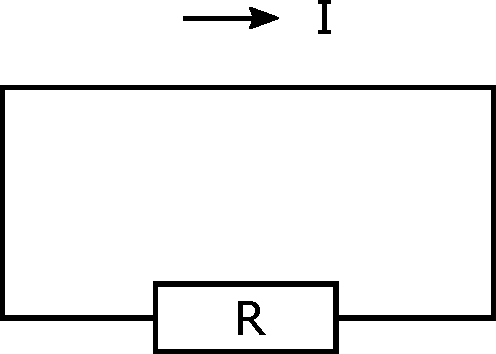
\includegraphics[width=0.9\linewidth]{Pics/shortedcircuit}
		\label{fig:shortedcircuit}
	\end{figure}
\end{minipage}
%
\hspace*{0.05\linewidth}
%
\begin{minipage}{0.48\linewidth}
	It was found that even a shorted circuit consisting of just one resistor does show a finite current, which is zero on average $\expval{I} = 0$, but has a non-zero fluctuation spectrum
	%
	\begin{equation}
	S_I^{(\omega)} = 2 \frac{k_B T}{R \pi}
	\end{equation}
	%
\end{minipage}
%
\\ 

Here, we assume the classical limit $\hbar \omega \ll k_B T$. The inverse resistance plays the role of a linear response coefficient $I = \frac{1}{R} U$.


\newpage
\section{FDT for classical systems}

%
\begin{figure}[H]
	\centering
	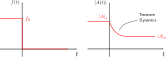
\includegraphics[width=0.9\linewidth]{Pics/derivationFDT}
	\label{fig:derivationfdt}
\end{figure}
%
Lets consider a system described by the Hamiltonian $H_1 = H_0 - f A$ for times $t < 0$, with the probability density $p_1(x) \sim \exp(- \beta H_1)$. At $t = 0$ we switch off the external field $f$ coupled to the observable $A$. Thus, $p(x,t) \to \exp(-\beta H_0)$ for $t \to \infty$. The ensemble-average of $A$ is given by $\expval{A} = \int{\dd{x} A(x) p(x,t)}$ and we integrate over microstates $x = (p_1, \dots, p_N, q_1, \dots, q_N)$. 

\begin{theorem}[Fluctuation Dissipation Theorem]
	%
	The FDT relates the fluctuation spectrum on the left side to the dissipative response to an external field on the right side of
	%
	\begin{equation}
	S_A(\omega) = \frac{2 k_B T}{\omega} \Im (\tilde{\chi}_A(\omega))
	\end{equation}
	%
\end{theorem}

In order to show that the Fluctuation Dissipation Theorem holds we need to key concepts:
%
\begin{itemize}
	\item{Boltzman distribution $p_0 \sim \exp(- \beta H_0)$ with $\beta = \frac{1}{k_B T}$}
	\item{time propagator $P(x_1, t_1 | x_0, t_0)$}
\end{itemize}

 
\subsection*{Fluctuation Spectrum}

The auto-correlation function is given by
%
\begin{equation}
	C_A(\tau) = \expval{A(t) A(t+\tau)} - \expval{A}^2
\end{equation}
%
which is independent of $t$ at thermal equilibrium. The correlation function is an even function $C_A(\tau) = C_A(-\tau)$. It is related to the time propagator by 
%
\begin{equation}
C_A(\tau) = \int \dd{x_0} \dd{x_1} A(x_0) A(x_1) p_0(x_0) P(x_1, t+\tau | x_0, t) - \expval{A}^2
\end{equation}
%

The power spectral density is then the Fourier transform
%
\begin{equation}
	S_A(\omega) = \tilde{C}_A(\omega) = \int \dd{\tau} C_A(\tau) e^{i \omega \tau}
\end{equation}
%
where we use the non-unitary Fourier transform with angular frequency. 
%
\begin{theorem}[Wiener-Kinchin Theorem]
	The Fourier transform exists and has the usual properties.
\end{theorem}
%
Formally, we have $\expval{\tilde{A}(\omega) \tilde{A}^*(\omega')} = S_A(\omega) \delta(\omega - \omega')$. Note, however that $\tilde{A}(\omega)$ is not in a strict mathematical sense defined.

\subsection*{Linear Response Function}

Let a system possess the Hamiltonian $H(x,t) = H_0(x) - A(x) f(t)$. Then, the linear response is expressed by
%
\begin{equation}
	\expval{A(t)} = \expval{A}_0 + \int_{-\infty}^{\infty} \dd{\tau} \chi_A(\tau) f(t-\tau) + \O{f^2}
\end{equation}
%
which defines the linear response function $\chi_A(\tau)$. Causality implies that $\chi_A(\tau) = 0$ for all $\tau < 0$.

The Fourier transform reads
%
\begin{equation}
\tilde{\chi}_A(\omega) = \int_{-\infty}^{\infty} \dd{\tau} \chi_A(\tau) e^{i \omega \tau}
\end{equation}
%

\subsection*{Example: Oscillating Field}
%
\begin{equation}
	f(t) = f_0 \cos(\omega t) = \Re f_0 e^{i \omega t}
\end{equation}
%
then
%
\begin{equation}
	\expval{A(t)} = \expval{A}_0 + [\Re \tilde{\chi}_A(\omega)] f_0 \cos(\omega t) - [\Im \tilde{\chi}_A(\omega)] f_0 \sin(\omega t)
\end{equation}
%
so $f(t)$ oscillates with the frequency of driving with amplitude $f_0 |\tilde{\chi_A(\omega)}|$ and with phase lag $\arg(\tilde{\chi_A(\omega)})$. The power performed by the external field is given by $R = - f(t) \dv{t} A(x(t))$ with the time-average $\expval{R} = \frac{1}{2} \omega f_0^2 \Im \tilde{\chi_A(\omega)}$. Thus, the imaginary part $\Im \tilde{\chi}_A(\omega)$ characterises the dissipative response of the system.

\subsection*{Derivation of the fluctuation-dissipation-theorem}

Let $f(t) = f_0 \Theta(-t)$. We first compute the partition function $Z_1 = \int \dd{x} \exp{- \beta H_1}$ with 
%
\begin{equation}
	f_1(x) = \frac{1}{Z_1} \exp{- \beta H_1} \approx p_0(x) [1 + \beta f_0(A(x) - \expval{A}_0)]
\end{equation}
%
For $t \geq 0$ we have 
%
\begin{align*}
\expval{A(t)} &= \int \dd{x} A(x) p(x,t) = \int \dd{x} A(x) \int \dd{x_0} P(x, t | x_0, t_0) p_1(x_0) \\
&= \int \dd{x} A(x) \int \dd{x_0} P(x, t | x_0, t_0) p_0(x_0) [1 + \beta f_0 A(x) - \beta f_0  \expval{A}_0] \\
&= \expval{A}_0 + \beta f_0 \expval{A(t) A(0)} -\beta f_0 \expval{A}^2_0 \\
&= \expval{A}_0 + \beta f_0 C_A(t)
\end{align*}
%
We also know that
%
\begin{equation}
\expval{A(t)} = \expval{A}_0 + \int_{-\infty}^{\infty} \dd{\tau} \chi_A(\tau) f(t-\tau)
\end{equation}
%
The derivative with respect to time reads
%
\begin{equation*}
	\chi_A(t) = 
	\begin{cases} 
		\beta \dv{t} C_A(t) & for \quad t \geq 0 \\ 
		0 & for \quad t < 0
	\end{cases}
\end{equation*}
%

%
\begin{remark}[Remark: Even and Odd Functions]
	%
	Every function $F(t)$ can be separated into an even and an odd part
	%
	\begin{equation*}
	F(t) = 
	\begin{cases} 
	F'(t) = \frac{1}{2} [F(t) + F(-t)] \, (\mathrm{even}) \quad \Rightarrow & \tilde{F}'(\omega) = \Re \tilde{F}(\omega) \\ 
	F''(t) = \frac{1}{2} [F(t) - F(-t)] \, (\mathrm{odd}) \quad \Rightarrow & \tilde{F}'(\omega) = i \Im \tilde{F}(\omega)
	\end{cases}
	\end{equation*}
	%
	\underline{Caution:} The prime $'$ indicates the even part, not a derivative!
	%
\end{remark}
%

so $C_A(t)$ is even, thus $\dv{t} C_A(t)$ is odd and as we take only the odd parts 
$\chi_A''(t) = \frac{1}{2} \beta \dv{t} C_A(t)$
and so $i \Im \tilde{\chi}_A(\omega) = \frac{1}{2} \beta (+ i \omega) \delta_A(\omega)$

In classical mechanics we have $\frac{1}{\beta} = k_B T$, in quantum mechanics we have $\hbar \omega = \coth \frac{\beta \hbar \omega}{2}$

\subsection*{Example: Optical Trap}

An optical trap can be described by 
%
\begin{equation}
	k x + \gamma \dot{x} = \gamma \xi(t) \quad \mathrm{with} \quad \expval{\xi(t)} = 0
\end{equation}
%
The fluctuation dissipation theorem is telling us that
%
\begin{equation}
	S_x(\omega) = \frac{2 k_B T}{\omega} \Im \tilde{\chi}_x(\omega) = \frac{2 k_B T / \gamma}{(k/\gamma)^2 + \omega^2}
\end{equation}
%
Thus, one can  estimate $k$ by measuring $S_x(\omega)$. As a generalised example, we consider
%
\begin{equation}
	\sum_{k = 0}^n a_k x^{(k)}(t) = \xi(t)
\end{equation}
%
for which we do a a Fourier transformation in order to get
%
\begin{equation}
	\underbrace{\sum_{k = 0}^n a_k (i \omega)^k}_{= \tilde{\chi}^{-1}_A(\omega)} \tilde{\chi}(\omega) = \tilde{\xi}(\omega)
\end{equation}
%
so
%
\begin{align*}
	& \tilde{\chi}(t) = \tilde{\chi}_A(t) \tilde{\xi}(\omega) \\
	& \chi(t) = \int_0^{\infty} \dd{\tau} \tilde{\chi_A}(\tau) \xi(t-\tau)
\end{align*}
%
We have
%
\begin{align*}
S_x(\omega) \delta(\omega - \omega') &= \expval{\tilde{\chi}(\omega)\tilde{\chi}^*(\omega')} \\ 
&= \tilde{\chi}_A(\omega) \tilde{\chi}^*_A(\omega') \expval{\tilde{\xi}(\omega) \tilde{\xi}(\omega')} \\
&= |\tilde{\chi}_A(\omega)|^2 2D \delta(\omega - \omega')
\end{align*}
%
so 
%
\begin{equation}
	S_x(\omega) = |\tilde{\chi}_A(\omega)|^2 2D = \frac{2 k_B T}{\omega} \Im \tilde{\chi}_A(\omega)
\end{equation}
%
%
\begin{equation}
	2D = \frac{2 k_B T}{\omega} \frac{\Im \tilde{\chi}_A(\omega)}{|\tilde{\chi}_A(\omega)|^2}
\end{equation}
%
For the special case $a_1 = \gamma$, but $(a_{2k+1} = 0)$ for $k > 0$ we have
%
\begin{equation}
	\tilde{\chi}_A = \frac{1}{R(\omega) - i \omega \gamma} \quad \Rightarrow \quad \Im \tilde{\chi}_A = \frac{\omega \gamma}{R^2(\omega) + \omega^2 \gamma^2}
\end{equation}
%
Thus, $D = k_B T \gamma$

\chapter{A Link to Statistical Physics}

The fluctuation-dissipation theorem is a hallmark of equilibrium systems. Living systems can violate the fluctuation-dissipation theorem. 

\section{Detailed Balance}

A system that can reach equilibrium andhas a zero net current at equilibrium obeys to so-called detailed balance. It means, that it is not possible to distinguish whether a dynamics is played forwards or backwards in time. It defines reversible Markov chains.

We can formulate the condition of detailed balance both for continuous and discrete state space descriptions.

\begin{theorem}[Condition for Detailed Balance]
	%
	We say the dynamics obeys "detailed balance" if
	%
	\begin{itemize}
		\item{there exists an equilibrium distribution $P^*$ or $P_j^*$ in the discrete case}
		\item{the joint probability is symmetric $P^*(x', \tau | x, 0) = P^*(x, \tau | x', 0)$ and $P^*(i, \tau | j, 0) = P^*(j, \tau | i, 0)$ / $L_{ji} P_j^* = L_{i,j} P_i^*$, respectively}
	\end{itemize}
	%
	Its behaviour is governed for continuous state space by the Fokker-Planck equation
	%
	\begin{equation}
		\dv{t} p(x,t) = \hat{L} p(x,t)
	\end{equation}
	%
	and for discrete state space by the Master equation
	%
	\begin{equation}
		\dv{t} P_j(t) = P_i(t) L_{ij}
	\end{equation}
	%
\end{theorem}

This means that there is zero net current at equilibrium $i \rightleftharpoons j$. So for example if the transition matrix is symmetric a system obeys detailed balance.

\subsection*{Example: Boltzmann distribution}

A simple example is the Boltzmann distribution for a canonical ensemble, where you have states $0, 1, 2, \dots$ with energies $E_0, E_1, E_2, \dots$ so
%
\begin{equation}
	P_i^* = \frac{1}{Z} \exp(- \beta E_i)
\end{equation}
%
and
%
\begin{equation}
	\frac{L_{ji}}{L_{ij}} = \exp(- \beta (E_i - E_j))
\end{equation}
%
A counter example would be a circular current $1 \rightarrow 2 \rightarrow 3 \rightarrow 1$ with rate $r$ giving
%
\begin{equation}
	\hat{L} = \begin{pmatrix}
	-r & r & 0 \\
	0 & -r & r \\
	r & 0 & -r
	\end{pmatrix}
\end{equation}
%
with eigenvalue $\lambda_1 = 0$ with corresponding eigenvector $ \vec{e}_1 = \left(\frac{1}{3}, \frac{1}{3}, \frac{1}{3} \right)^T $ and $\lambda_2 = \lambda^*_3 = \left(-\frac{3}{2} + i \frac{\sqrt{3}}{2} \right) r$ resulting in a net current at equilibrium, thus breaking detailed balance. 

\subsection*{Proof of Detailed Balance for Hamiltonian Systems}

We consider a system characterised by some Hamiltonian $H$ obeying the Hamilton equations
%
\begin{equation}
\dot{p}_i = -\pdv{H}{q_i} \quad \dot{q}_i = \pdv{H}{p_i}
\end{equation}
%
with the macroscopic observable $y = Y(q,p)$. The detailed balance holds if
%
\begin{itemize}
	\item[(i)]{$H$ is even in $p_i$}
	\item[(ii)]{$Y$ is even in $p_i$}
\end{itemize}
%
Then the time propagator $T$ fulfills the condition
%
\begin{equation}
	P(y',\tau | y, 0) = T_{\tau}(y'|y)P^*(y) = T_{\tau}(y|y')P^*(y') = P(y,\tau | y', 0)
\end{equation}
% 

%
\begin{remark}[Nota Bene]
	We always have
	%
	\begin{equation}
		T_{\tau}(y'|y)P^*(y) = T_{-\tau}(y|y')P^*(y)
	\end{equation}
	% 	
	as we can play backwards the dynamics in time.
\end{remark}
%

%
\begin{figure}[H]
	\centering
	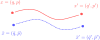
\includegraphics[width=0.7\linewidth]{Pics/timereversal}
	\label{fig:timereversal}
\end{figure}
%
For the proof of this we make use of time reversal notation
%
\begin{equation}
	\bar{t} = -t \quad \bar{q}_i = q_i \quad \bar{p}_i = -p_i
\end{equation}
%
We start by looking at a trajectory in $(q,p)$-phase space and for every point $x' = (q', p')$ we apply time reversal $\bar{x}' = (\bar{q}', \bar{p}')$. By (i) we conclude that $H(x) = H(\bar{x})$ and thus $P^*(x) = P^*(\bar{x})$ (even in $p_i$ means in our case symmetric in time!). Also, we have $X = Y^{-1}(y)$ and by (ii) $X = \bar{X}$ as $Y$ is even. 

\begin{figure}[H]
	\centering
	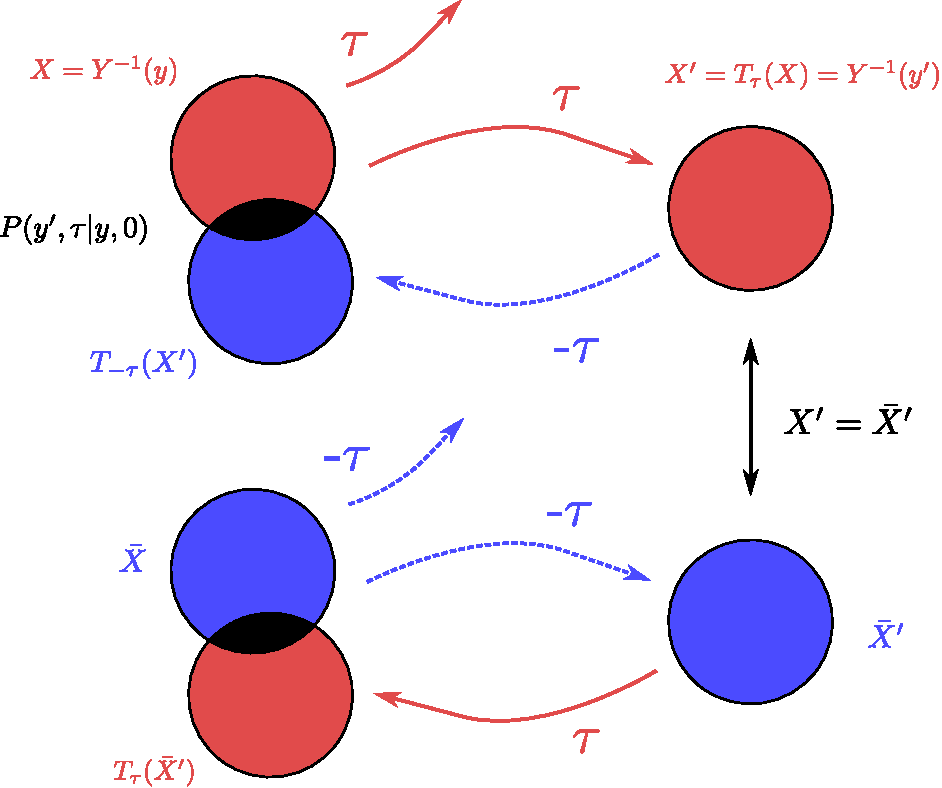
\includegraphics[width=0.9\linewidth]{Pics/detailedbalance}
	\label{fig:detailedbalance}
\end{figure}

We can express the probability to observe $y'$ at time $\tau$ after observing $y$ at time $0$ by the integral over the phase space region $X \cap T_{-\tau}(X')$ of the equilibrium probabilities $P^*(x)$
%
\begin{equation*}
T_{\tau}(y'|y) P^*(y) = P(y',\tau | y,0) = \int_{X \cap T_{-\tau}(X')} \dd{x} P^*(x) 	
\end{equation*}
%
As we have $P^*(x) = P^*(\bar{x})$ we can also change the area of integration in phase space to $\overline{X \cap T_{-\tau}(X')}$
%
\begin{equation*}
\int_{X \cap T_{-\tau}(X')} \dd{x} P^*(x) = \int_{\overline{X \cap T_{-\tau}(X')}} \dd{x} P^*(x)
\end{equation*}
%
From the diagram above we see that the states in the lower red circle $T_{\tau}(\bar{X}')$ are mapped to the states in the upper blue circle $T_{-\tau}(X')$ under time reversal
%
\begin{equation}
	\overline{T_{-\tau}(X')} = T_{\tau}(\bar{X}')
\end{equation}
%
and so we have
%
\begin{equation}
	\overline{X \cap T_{-\tau}(X')} = \bar{X} \cap \overline{T_{-\tau}(X')} = \bar{X} \cap T_{\tau}(\bar{X}') = X \cap T_{\tau}(X')
\end{equation}
% 
We conclude
%
\begin{equation}
\int_{\overline{X \cap T_{-\tau}(X')}} \dd{x} P^*(x) 
	= \int_{X \cap T_{\tau}(X')} \dd{x} P^*(x) 
	= P(y, \tau | y', 0) = T_{\tau}(y|y') P^*(y')
\end{equation}
%
So at equilibrium we cannot distinguish whether a dynamics is played forward or backward in time.

\section{Increase of Relative Entropy}

We consider a Master equation for a Markov chain
%
\begin{equation}
	P_j^{(n+1)} = \sum_i{P_i^n \, T_{ij}}
\end{equation}
%
with the probability $P_i^n$ to be in state i at time $t = t_n$ and a matrix of transition probabilities $\left( T_{ij} \right)$ fulfilling $\sum T_{ij} = 1$. For a stationary distribution with $P_j^* > 0$ so that $P_j^* = \sum_i P_i^* \, T_{ij}$ for all $j$, we define the relative entropy (Kullberg-Leibler divergence) as
%
\begin{equation}
	D_n = K L(P^n||P^{-k}) = \sum P_i^n \ln \left( \frac{P_i^n}{P_i^*} \right)
\end{equation}
%
%
\begin{theorem}[Theorem]
	$D_{n+1} \leq D_n$
\end{theorem}
%
This theorem is a direct consequence of the convexity of $D_n$. For $P_i^* = \frac{1}{N}$, one finds that $D_n = -\sum P_i \ln(P_i) - \ln(N)$, i.e. the entropy increases with time.

\newpage

\section{Equilibrium vs Non-Equilibrium}

\subsection*{Signs of Equilibrium}

\begin{itemize}
	\item FDT
	\item detailed balance $L_{ji}P_j^* = L_{ij}P_i^*$
	\item equipartition theorem
\end{itemize}

All of these constrain the Langevin equation to approach thermal equilibrium. At equilibrium we have the Boltzmann distribution as a maximum entropy distribution. 

Let us consider a macrostate $y$ with microstates $x = Y^{-1}(y)$. For every probability distribution you can think of we can define the entropy
%
\begin{equation}
	S = \int p(x|y) \ln(p(x|y))
\end{equation}
%
that is the relative information of $x$ with respect to $y$ (dimensionless / natural units / units of bits). So $\frac{S}{\ln(2)}$ is the average number of yes / no questions to infer $x$ if only $y$ is known.

In information theory you define a piece of information as 1 nat = $\ln(2)^{-1}$ bits. Rescaling by $\ln(2)$ is equivalent to defining the entropy instead using the binary logarithm.

\subsection*{Properties of Non-Equilibrium Systems}

\begin{itemize}
	\item non-generic steady states possible (e.g. circular currents)
	\item small number of non-equilibrium fluctuation theorems is available
\end{itemize}

\subsection*{Derivation of the Boltzmann distribution}

Lets consider a system with $\expval{E} = U$ for the canonical ensemble, which is contact with some heath bath of temperature $T$. As a trick we map the it to a microcanonical ensemble of $N$ independent systems with $N_i$ system in an energy state $E_i$. 

Now we have two constraints:
%
\begin{itemize}
	\item[i)]  $\sum_i N_i = N$
	\item[ii)] $\sum_i N_i E_i = N U$
\end{itemize}
%

Then we introduce the weight function $W$ from statistical physics and count how many compatible microstates there are for a given set $\{ N_i \}$. Doing simple combinatorics we get
%
\begin{equation}
	W = \frac{N!}{N_1! N_2! \dots}
\end{equation}
%
The macrostate with maximum $W$ is most probable, but we need to take into account the constraints. So the way to go is to introduce Lagrange multipliers. We know that 
%
\begin{equation}
	0 = \dd{\ln(W)} = \sum_i \pdv{\ln(W)}{N_i} \dd{N_i} + \alpha \sum \dd{N_i} - \beta \sum E_i \dd{N_i}
\end{equation}
%
so
%
\begin{equation}
 \pdv{\ln(W)}{N_i} + \alpha - \beta E_i = 0
\end{equation}
%
with
%
\begin{equation}
\pdv{\ln(W)}{N_i} \overset{\mathrm{Stirling}}{=} \pdv{N_j \ln(N_j)}{N_i} - \sum_j \pdv{N \ln(N)}{N_i} = \dots = - \ln(\frac{N_i}{N})
\end{equation}
%
so $p_i = \frac{N_i}{N} = \exp(\alpha - \beta E_i)$. You can play this game also for the grand canonical ensemble with a third condition for the mean particle number.

\section{Thermal Fluctuations: Space-dependent Diffusion}

Our diffusion coefficient now depends on the position $D = D(x)$ and we write down a Langevin equation
%
\begin{equation}
	\gamma \dot{x} = - \pdv{U}{x} + \gamma \xi(t)
\end{equation}
%
and we have Gaussian white noise with a position-dependent noise strength $\expval{\xi(t)\xi(t')} = 2 D(x) \delta(t-t')$. So far we can't tell whether to use Stratonovich or Ito calculus.

Starting with the Einstein relation $D = \frac{k_B T}{\gamma}$ we can distinguish two cases: 

\begin{itemize}
	\item[i)] $\gamma = \gamma(x)$ and $T = T_0$ (equilibrium system, just passive obstacles by $\gamma$!)
	\item[ii)] $\gamma = \gamma_0$ and $T = T(x)$ (non-equilibrium system!)
\end{itemize}

\subsection*{$\alpha$-calculus}

$(\alpha) \, \dot{x} = f(x) + \alpha g(x)$ with $\alpha = 0$ for Ito and $\alpha = \frac{1}{2}$ for Stratonovich. This determines what the Fokker-Planck equation looks like
%
\begin{equation}
	\dot{P} = \pdv{x} \left[ -(f + \frac{\alpha}{2} \pdv[2]{g}{2})P + \frac{1}{2} \pdv{x} (g^2 P) \right]
\end{equation}
%

\subsection*{Case i): Equilibrium System}

For case i) it can be shown that $\alpha = 1$ is correct (isothermal interpretation) (see Lau \& Lubensky paper PRE).
%
\begin{equation}
\dot{P} = \pdv{x} \left[ -(f + \pdv[2]{g}{2})P + \frac{1}{2} \pdv{x} (g^2 P) \right]
\end{equation}
%
with $f = - \frac{1}{\gamma} \pdv{U}{x}$, $g = \sqrt{2D}$ so
%
\begin{equation}
\dot{P} = - \nab(fP) + \nab(D(x)\nab P)
\end{equation}
%
so this is the correct generalization of Fick's law for equilibrium systems with $\gamma = \gamma(x)$. So at the steady state we must have $\dot{P}^* = 0$ and $fP) + D(x)\nab P = \mathrm{const}$ and we get the Boltzmann distribution $P^* \sim \exp(-\beta U)$.

\begin{remark}[Nota Bene]
In Ito interpretation with $\alpha = 0$ we would have obtained the Fokker-Planck equation 
%
\begin{equation}
\dot{P} = - \nab(fP) + \nab^2(D P)
\end{equation}
%
which gives rise to different physics and different steady state distributions. So it is really important where to write $D$!
\end{remark}

\subsection*{Case ii): Position-dependent Temperature}

These systems behave non-generically and are characterized by thermophoreses (Sorret effect) and the Fokker-Planck equation
%
\begin{equation}
\dot{P} = - \nab(f -D_T \nab T)P + \nab(D(x)\nab P)
\end{equation}
%
with the Sorret coefficient $S_T = \frac{D_T}{D}$, which depends on molecular interaction potentials. The Sorret effect is an example of an non-equilibrium phenomenon. 

\section{Entropy Production}

A hallmark of non-equilibrium systems is entropy production, which we know from the second law of thermodynamics $\expval{\Delta S} \geq 0$.

As an example lets consider to systems of temperature $T_1$ and $T_2$ that are brought into contact resulting in an entropy change
%
\begin{equation}
	\frac{\Delta S}{k_B} = \Delta Q (\frac{1}{k_B T_2} - \frac{1}{k_B T_1})
\end{equation}
%
Or consider a second example of two ideal gases with $N_A$ and $N_B$ particles that are mixing: $N = N_A + N_B$, $x = \frac{N_A}{N}$ and 
%
\begin{equation}
	\frac{\Delta S}{k_B} = - N [x \ln(x) + (1-x)\ln(1-x)]
\end{equation}
%
as the mixing entropy.

\subsection*{Fluctuation Theorem of Non-Equilibrium Systems}

The change of entropy will be a stochastic variable with 
%
\begin{equation}
	\frac{P \left(\frac{\Delta S}{k_B} = I \right)}{P \left(\frac{\Delta S}{k_B} = -I \right)} = \exp(I)
\end{equation}
%
for a colloidal particle driven by optical tweezers a decrease in entropy might be observed, for larger system it gets really unlikely due to the exponential factor $\exp(I)$.

\subsection*{Crooke Fluctuation Theorem}

Lets consider a macroscopic observable $y$ so we can ask how likely it is to observe the time-reversed macroscopic dynamics / trajectory
%
\begin{equation}
\frac{P \left( y \right)}{P \left( \bar{y} \right)} = \exp(\Delta S[y(t)] / k_B)
\end{equation}
%

\subsection*{Jarzynski Relation}

For an isolated system there is always an adiabatic process connecting $y_0$ and $y_1$ costing the work $W = \Delta F$ as change in the free energy. Any non-adiabatic process will take more work $\expval{\Delta F} \leq W$ and we have
%
\begin{equation}
	\exp(- \Delta F) = \expval{\exp(-\beta W)}
\end{equation}
%

\chapter{Decision Theory}

Consider a (biomedical) variable $z$ which will have different statistics $P(z|s_1)$ and $P(z|s_2)$, respectively, for the two states $s_1$ meaning "healthy" and $s_2$ meaning "'ill"'.

So our task is now to decide between the options $d_1$(guess $s_1$) and $d_2$(guess $s_2$). So we can have a look at the likelihood ration
%
\begin{equation}
	\Lambda = \frac{P(z|s_1)}{P(z|s_2)}
\end{equation}
%
and employ a maximum-likelihood test

to decide for $d_1$ if $P(z|s_1) > P(z|s_2)$, i.e. $\Lambda > 1$
to decide for $d_2$ if $P(z|s_2) > P(z|s_1)$, i.e. $\Lambda < 1$

There are different types of errors

$P(d_2 | s_1)$ = Type-I error (false alarm / false positive error)

$P(d_1 | s_2)$ = Type-II error (false negative error / a building is burning, but the fire alarm is not set off)

Any statistical test can be characterized by its Receiver of Operating Characteristics (ROC)

\subsection*{Bayes Risk Criterium}

We have a cost matrix with $\hat{c} = \begin{pmatrix} c_{11} & c_{12} \\ c_{21} & c_{22} \end{pmatrix}$ and $c_{ij}$ cost of $d_i$ if $s_j$ true
$c_{12}$ cost of $d_1$ if $s_2$ true

and the base rates $P(s_1)$, $P(s_2) = 1-P(s_1)$

so now we can calculate an expected cost
%
\begin{equation}
	\expval{c} = c_{11} P(d_1|s_1) P(s_1) +  c_{12} P(d_1|s_2) P(s_2) + \dots
\end{equation}
%
so an optimal test for the likelihood ratio would be
%
\begin{equation}
\Lambda(z) = \frac{P(z|s_2)}{P(z|s_1)} \overset{d_1}{<} \overset{d_2}{>} \frac{(c_{21}-c_{11}) P(s_1)}{(c_{12}-c_{22}) P(s_2)} = \theta
\end{equation}
%

Example: $c_{12} \to \infty$ then $\theta \to 0$ and always $d_2$ is chosen

Lets calculate an expected cost for the optimal test, so depending on the base probability $P_0 = P(s_2)$ what is the cost $c(P_0)$? --> GRAPHICS

Generalizations 

\begin{itemize}
	\item vector observations with $z_1$, $z_2$
	\item multiple decisions
\end{itemize}

\subsection*{Sequential Bayes Test}

We can either decide for $d_1$, $d_2$ or $?$ which means undecided.

When zero measurements are made we have
%
\begin{equation}
	\Lambda_0 = \frac{P(s_2)}{P(s_1)}
\end{equation}
%
Without loss of generality we can write  $\hat{c} = \begin{pmatrix} 0 & c_{12} \\ c_{21} & 0 \end{pmatrix}$ (only the differences are relevant)

Question: So would it be beneficial to take one more measurement?

with $Q_1$, $Q_2$ are the critical base rates so that $c_{12} Q_1 = c(Q_1) + \beta$ and $c_{21} (1-Q_2) = c(Q_2) + \beta$

(Left side: cost for no measurement, right side: cost for one measurement)

$T_1 = \frac{Q_1}{1-Q_1}$ and $T_2 = \frac{Q_2}{1-Q_2}$ (corresponding likelihood ratios)

If $\Lambda_0 < T_1$ then we go for $d_1$, if $\Lambda_0 > T_2$ then $d_2$ and if in between then we take another test.

Next step: one measurement, so we can calculate an updated likelihood ratio 
%
\begin{equation}
\Lambda_1(z_1) = \frac{P_1}{1-P_1} = \frac{P(s_2|z_1)}{P(s_1|z_1)} = \frac{P(z_1|s_2)P(s_2)}{P(z_1|s_1) P(s_1)} = \frac{P(z_1|s_2)}{P(z_1|s_1)} \Lambda_0
\end{equation}
%
so if $\Lambda_1 < T_1$ then $d_1$, if $\Lambda_1 > T_2$ then $d_2$ and if $T_1 \geq \Lambda_1 \geq T_2$ we perform the second measurement with
%
\begin{equation}
\Lambda_2(z_2) = \frac{z_2|s_2}{z_2|s_1} \Lambda_1
\end{equation}
%

So the assumptions are, that measurements are independent and identically distributed. So from the sequential test we get $z_1$, $z_2$, $z_3$ ...

\section{Statistical Testing}

Decision theory meant, that we have a number of different measurement models and we decide which one is more likely. 

For statistical testing usually we have a working hypothesis $H_1$ and this can be formulated just qualitatively. Like $H_1 = $ "Smoking promotes cancer.", but we don't have a measurement model. 

But we can look at the Null hypothesis, i.e. the negation of our working hypothesis, $H_0 = \neg H_1$ for which we have a measurement modell $P(z)$ with measurement $z$ if $H_0$ true.

For the statistical test we have a decision problem, where in the first step we accept the Null hypothesis as $d_1$ and reject it as $d_2$. And we would like to formulate a decision rule, so that for a measurement $z_0$ we have $P(z \geq z_0) \overset{d_2}{<} \overset{d_1}{>} \alpha$ with the significance level $\alpha$.

Look elsewhere fallacy: if we were testing $n$ null hypothesis $H_0^{(1)}$, $H_0^{(2)}$, ..., $H_0^{(n)}$ with fixed $\alpha$ then even if $H_0^{(j)}$ are true for all $j$ an average of $\alpha n$ null hypothesis will be rejected. 

one-sided / two-sided tests: 

$\int_{\theta}^{\infty} P(z) \dd{z} \overset{d_2}{<} \overset{d_1}{>} \alpha$ one-sided

$\int_{|z| \geq \theta} P(z) \dd{z} \overset{d_2}{<} \overset{d_1}{>} \alpha$ two-sided

So when to go for a one-sided or two-sided test? Here the working hypothesis $H_1$ comes in 

Example fair coin: $H_0$ with $p_{\mathrm{head}} = p_{\mathrm{tail}} = 1/2$

measurement: $k$-times tail after tossing $n$-times, so we have a measurement model

So the probability is $p(k) = 2^{-n} \binom{n}{k}$

For a one-sided test ($H_0$: We have a biased coin towards tail) we have

$\sum_{k=k_1}^n p(k) \overset{d_2}{<} \overset{d_1}{>} \alpha$

and for a two-sided test ($H_0$: we have unknown bias) we have

$\sum_{k=k_1}^n p(k) + \sum_{k=1}^{n-k_1} p(k) \overset{d_2}{<} \overset{d_1}{>} \alpha$

\section{Student's t-test}

$H_0$: $\expval{x} = \mu$ with measurement model $z = x \sim N(\mu, \sigma^2)$ with $\sigma^2$ unknown

A measurement now consists of $z_1$, ..., $z_n$ and
%
\begin{equation}
	t = \frac{\bar{z}-\mu}{\hat{\sigma}/\sqrt{n}}
\end{equation}
%
so the empirical mean $\bar{z} = \frac{1}{n}(z_1 + \dots + z_n)$ and $\hat{\sigma}^2 = \frac{1}{n-1}\sum_i (z_j-\bar{z})^2$

Nota Bene: $\bar{z} \sim N(\mu, \frac{\sigma^2}{n})$ and $\frac{\bar{z}-\mu}{\sigma/\sqrt{n}} \sim N(0,1)$

so the statistic of $t$ is independent of $\mu$, $\sigma^2$

The first strategy would be to perform stochastic simulations

The strategy number 2 would be to derive an analytical formula, so one can show $\bar{z}-\mu \sim N(0,\frac{\sigma^2}{n})$ and $\hat{\sigma}^2 \sim \sigma^2 \frac{\chi^2(n-1)}{n-1}$

def. $\chi^2$-distribution: $y_1$, ..., $y_n$ $\in$ $N(0,1)$ so

%
\begin{equation}
	Q = \sum_{j=1}^{n-1} y_j^2 \sim \chi^2(n-1)
\end{equation}
%

Note: $\bar{z}$ and $\hat{\sigma}^2$ are independent

def. t-distribution

The case that $t = \frac{A}{B}$ with $A \sim N(0,1)$ and $B \sim \chi^2(n-1)$

so Student went through all the algebra

\section{Fischer's Exact: Testing categorial data for correlations}

Lets consider the two categorial properties
%
\begin{itemize}
	\item[(A)]{e.g. person has been skmoking}
	\item[(B)]{e.g. person has cancer}
\end{itemize}
%

So the doctor compiles a continguency table of absolute frequencies

%
\begin{tabular}{c | c | c | c}
			& A 				& $\bar{A}$ 			& \\ \hline
B 			& $N_{AB}$ 			& $N_{\bar{A}B}$ 		& $N_B$ \\
$\bar{B}$ 	&	$N_{A\bar{B}}$ 	& $N_{\bar{A}\bar{B}}$ 	& $N_{\bar{B}}$
\end{tabular}
%

So our Null hypothesis $H_0$ reads: $p(B|A) = p(B)$

simplification: $N_A$, $N_B$ and $N$ are fixed, so there is a single degree of freedom $N_{AB}$

measurement model: pick $N_A$ objects at random and then count objects with A in selection

hypergeometric distribution
%
\begin{equation}
	p(N_{AB}) = \frac{\binom{N_B}{N_{AB}} \binom{N_B}{N_A-N_{AB}}}{\binom{N}{N_A}}
\end{equation}
%

N.B.: with replacement: Binomial Distribution
without relacement: Hypergeometric Distribution

one-sided test: (suppose $k > \frac{N_A}{N}N_B$) 
%
\begin{equation}
	\sum_{n = N_{AB}}^{N_A} p(k) < \alpha
\end{equation}
%

\section{Estimation Theory}

We have a measurement model with $p(z|x)$ with the measurement $z$ and some unknown parameter $x$.

Maximum-likelihood estimate: $\hat{x} = argmax p(z|x)$

later: Bayesian prior $p(x)$

\subsection*{Warm-Up Example}

How to combine noisy measurements? Suppose we have two methods 1 and 2 to measure x.

we have $p(z_1|x) \sim N(x,\sigma_1^2)$ and $p(z_2|x) \sim N(x,\sigma_2^2)$

Maximum-likelihood estimate for x:

$p(z_1,z_2|x) = p(z_1|x)p(z_2|x) \to max$

we take a product of two Gaussians and get the weighted mean
%
\begin{equation}
	\hat{x} = \frac{\sigma_2^2}{\sigma_1^2 + \sigma_2^2} z_1 + \frac{\sigma_1^2}{\sigma_1^2 + \sigma_2^2} z_2
\end{equation}
%

\subsection*{Bayes formula}

%
\begin{equation}
P(x|z) = \frac{P(z|x) P(x)}{P(z)}
\end{equation}
%

$P(x)$: prior knowledge, 
$P(z) = \int P(z|x) P(x) \dd{x} $ 
$P(z|x)$: measurement model,
$P(x|z)$: a-posteriori probability distribution

Example:

$P(x) \sim N(0,\sigma^2)$,
$P(z|x) \sim N(x,\theta^2)$
$P(z) \sim N(0,\sigma^2 + \theta^2)$
$P(x|z) \sim N(\hat{x}, \rho^2)$ 

with $\hat{x} = \frac{1}{1+\frac{\theta^2}{\sigma^2}} z = \frac{\theta^2}{\sigma^2 + theta^2} 0 + \frac{\sigma^2}{\sigma^2 + theta^2} z$

$\rho^2 = \frac{1}{\frac{1}{\sigma^2} + \frac{1}{\theta^2}}$

\subsection*{Curve Fitting as Estimation Problem}

data points: $x_i = f(\alpha)$ with unknown parameter $\alpha$

suppose we have just a set of noisy measurements $z_i = x_i + \xi_i \sim N(x_i,\sigma_i^2)$

Now we can ask for the likelihood for an observation: 

$P({z_i}|\alpha) \to max$ for $\alpha = \hat{\alpha}$

Assume: all measurements independent of each other

$P(\{z_i\}|\alpha) = \prod_{i=1}^k N_{z_i}(f_i(\alpha, \sigma^2)) \sim \exp[-\sum_{i=1}^k \frac{(f_i(\alpha) - z_i)^2}{2 \sigma^2}]$

so $\hat{\alpha}$ minimizes th sum of square errors $\sum_{i=1}^k (f_i(\alpha) - z_i)^2$

so this is equivalent to a least-square fit

Generalizations:

 - suppose we have different $\sigma_i^2$: weighted least-square fit, weight is $1/\sigma_i^2$
 
 - suppose we have non-Gaussian noise in our measurement model: do maximum likelihood estimate that maximize $P(\{z_i\}|\alpha)$
 
\section{Kalman Filters}

We have a state space $\vec{x}_k = \vec{x}(t_k)$ e.g. position and velocity of a spaceship. 

Previous estimate for $\hat{x}_{k-1}$ with covariance ellipse and then we can propagate our model forward obtaining $\hat{x}_k$

so at  every time step: how to combine the previous estimate and the new measurement optimally?

Notation:

$\hat{x}_{k-1|k-1}$: previous estimate of state at time $t_{k-1}$
$P_{k-1|k-1}$: covariance matrix of this estimate

predict step

$\hat{x}_{k|k-1}$: a-priori estimate of state at time $t_{k}$
$P_{k|k-1}$: covariance matrix of this estimate

measurement step: $z_k$

combined into: update step htta provides a weighted average 
$\hat{x}_{k|k}$ a-priori estimate
$P_{k|k}$: covariance matrix


Process Model: describes time evolution of our system / assume linear dynamics

$\vec{x}_{k} = \hat{F}_{k} \cdot \vec{x}_{k-1} + \vec{w}_k$

with the time-propagator $\hat{F}_{k}$ and the process noise $\vec{w}_k \sim N(0,\hat{Q}_k)$

Measurement Model

$\vec{z}_k = \hat{H}_k \cdot \vec{x}_k + \vec{v}_k$

measurement matrix $\hat{H}_k$
measurement noise $\vec{v}_k \sim N(0,\hat{R}_k)$

N.B. without loss of generality we can set $\hat{H} = $

Prediction Step

$\hat{x}_{k|k-1} = \hat{F}_{k} \cdot \vec{x}_{k-1|k-1}$
$P_{k|k-1} = \hat{F}_{k} P_{k-1|k-1} \hat{F}^T_{k} + \hat{Q}_k$

Measure $\vec{z}_k$

pre-fit residual / innovation $\vec{y}_k = \vec{z}_k - \hat{H}_k \cdot \vec{x}_{k|k-1}$

covariance pf $\vec{y}_k$: $\hat{S}_k = \hat{R}_k + \hat{H}_k P_{k|k-1} \hat{H}^T_k$

Update Step

$\hat{x}_{k|k} = \hat{x}_{k|k-1} + \hat{K}_k \vec{y}_k$ weighted average

$P_{k|k} = (\hat{I} - \hat{K}_k \hat{H}_k) P_{k|k-1} (\hat{I} - \hat{K}_k \hat{H}_k)^T + \hat{K}_k \hat{R}_k \hat{K}^T_k$

Optimal Kalman Gain

$\hat{K}_k = P_{k|k-1} \hat{H}^T_k \hat{S}^{-1}_k$

generalizes the warm-up example as ration of covariances

Theorem

The optimal Kalman gain has the following property: it minimizes the expectation value of the $L^2$-norm $E || \vec{x}_k - \hat{\vec{x}}_{k|k} ||^2$

Proof

$E || \vec{x}_k - \hat{\vec{x}}_{k|k} ||^2 = tr \hat{P}_{k|k}$

so

$0 =! \pdv{tr \hat{P}_{k|k}}{\hat{K}_k}$

so

$\pdv{tr AB}{A} = B^T$ because $\left( \pdv{tr AB}{A} \right)_{ij} = \pdv{tr AB}{A_{ij}} = \pdv{tr \sum_k (AB)_{kk}}{A_{ij}} = \pdv{tr \sum_{k,l} A_{kl}A_{lk}}{A_{ij}} = B_j$

similarly: $\pdv{tr BA^T}{A} = B$

Now: $tr \hat{P}_{k|k} = tr \hat{P}_{k|k-1} - \hat{K}_k \hat{H}_k \hat{P}_{k|k-1} - \hat{P}_{k|k-1}(\hat{K}_k \hat{H}_k)^T 
+ \hat{K}_k \hat{H}_k \hat{P}_{k|k-1} (\hat{K}_k \hat{H}_k)^T + \hat{K}_k \hat{R}_k\hat{K}^T_k$

$\pdv{tr P_{k|k}}{\hat{K}_k} = - 2 \hat{P}^T_{k|k-1} \hat{H}_k + 2 \hat{K}_k \hat{S}_k$

\chapter{Stochastic Resonance}

This is an example where noise plays a beneficial role for the detection of noisy oscillatory signals. We will consider a minimal model: Consider diffusion in a double-well potential $U_0 = - \frac{x^2}{2} + \frac{x^4}{4}$ and add weak periodic driving $U = U_0 + A \cos(\Omega t)$ as an input signal. 

Consider over-damped stochastic dynamics
%
\begin{equation}
	\dot{x} = -\pdv{U}{x} + \xi, \quad \expval{\xi(t) \xi(t')} = 2 D \delta(t-t')
\end{equation}
%
Remember the Kramer escape rates
%
\begin{equation}
	r_0 = \frac{1}{2 \pi} \sqrt{|U_0''(0)| U_0''(1)} \exp(-\frac{\Delta U_0}{D}) = \frac{\sqrt{2}}{2 \pi} \exp(-\frac{1}{4D})
\end{equation}
%
The stead-state distribution is a Boltzman distribution. Next look at the largest negative eigenvalue $\lambda_1 = \approx -r_0$, i.e. the slowest decaying mode. 

We can coarse-grain the stochastic process on a two state (telegraph) process, i.e. $x \approx -1 \leftrightarrow x \approx +1$ with a time scale given by the rates ging from left to the right $r_1(n_- \to n_+)$ and back $r_2(n_- \to n_+)$
and due to particle number conservation we have $\dot{n}_+ = -\dot{n}_- = r_- n_- - r_+ n_+ = r_-(r_+ + r_-) n_+$ so e can write down a formal solution
%
\begin{equation}
	n_+(t) = \exp(-\int_{t_0}^t \dd{t'} r) n_+(t_0) + \exp(-\int_{t_0}^t \dd{t'} r) \int_{t_0}^t \dd{t'} r(t') \exp(\int_{t_0}^{t'} \dd{t''} r)
\end{equation}
%
So lets apply this to the case $U = U(t)$ and to simplify our life we will assume $A \ll D$
%
\begin{equation}
r_{\pm}0 = \frac{\sqrt{2}}{2 \pi} \exp(-\frac{1}{4D} \mp \frac{A}{D} \cos(\Omega t))= \approx r_0 \left(1 \mp \frac{A}{D} \cos(\Omega t) \right)
\end{equation}
%
So if we insert this in the expression for $n_+$ we get
%
\begin{align*}
n_+(t) =& \exp(-2r_0 (t-t_0)) [n(t_0) + \frac{1}{2} \exp(2 r_0 (t-t_0) - 1) \\
&+ \frac{r_1}{\sqrt{\Omega^2 + 4r_0^2}} \cos(\Omega t - \varphi) \exp(2r_0(t-t_0) - \cos(\Omega t-\varphi))]
\end{align*}
%
with $r_1 = \frac{r_0 A}{D}$ and $\tan(\varphi) = \frac{\Omega}{2 r_0}$ and for $t \gg t_0$ we get
%
\begin{equation}
n_+ = \frac{1}{2} + \frac{r_1}{\sqrt{\Omega^2 + 4r_0^2}} \cos(\Omega t - \varphi)
\end{equation}
%

Next we look at the autocorrelation function of this process
%
\begin{equation}
	\expval{x(t)} = x_+ p_+(t) + x_- p_-(t) = p_+(t) - p_-(t)
\end{equation}
%
with $x_{\pm} = \pm 1$ and $p_+ = n_+ / n$ and so we get
%
\begin{align*}
	\expval{x(t) x(t+\tau) | x_0, t_0} &= \sum_{s,s'} s \cdot s' P(s,t+\tau | s', t) P(s',t|x_0,t_0) \\
	&= p_+(t+\tau | +1, t) p_+(+1, t|x_0,t_o) + \dots
\end{align*}
%
(take all combinations $11, 1-1, -11,-1-1$)

We use $p_p = 1-p_+$ and consider the limit $t_0 \to -\infty$, thus
%
\begin{align*}
	\expval{x(t) x(t+\tau)} =& \exp(-2 r_0 \tau) + 2 r_1 \\
	&+ 4 r_1^2 [\exp(-2 r_0 \tau) \cos^2(\Omega t - \varphi) + \cos(\Omega (t+\tau) - \varphi) \cos(\Omega t - \varphi)]
\end{align*}
%
Now the autocorrelation function depends on time, as this is not just a static process, i.e. time translation symmetry is broken. Note that is only depends on $\Omega t \% 2 \pi$, so it doesn't matter which cycle of driving is chosen.

If we average over $t$ we get
%
\begin{equation}
	C(\tau) = 	\expval{x(t) x(t+\tau)}_t = \exp(-2r_0 |\tau|) [1 - 2 r_1^2] + 2 r_1^2 \cos(\Omega t)
\end{equation}
%
with a decaying and periodic component. We get the power spectral density be doing a Fourier transform by the Wiener-Klinchine theorem
%
\begin{equation}
S(\omega) = F(C(\tau)) = (1- 2 r_1^2) \frac{4 r_0}{4 r_0^2 + \omega^2} + 2 \pi r_1^2 (\delta(\omega-\Omega) + \delta(\omega + \Omega))
\end{equation}
%
The first term determines the noise contribution (decaying term / a Lorentzian) and the second term represents the periodic contribution. So one defines the signal-to-noise ration
%
\begin{equation}
SNR = \frac{S}{B} = \pi \frac{r_1^2}{r_0} = \frac{1}{\sqrt{2}} \frac{A^2}{D^2} \exp(-\frac{1}{4 D})
\end{equation}
%
So our signal is better, if we have some noise in our system! The SNR attains a maximum at a finite $D$ (before the decay with $D^{-2}$). This can be intuitively understood that for $\frac{1}{r} = \frac{1}{2} T = \frac{1}{2} \frac{2 \pi}{\Omega}$ then the particle is jumping according to the oscillatory change in the potential. 

Glimpse on Infotaxis: Infotaxis as a strategy for searching without gradients by Vergassola 2007


\nocite{*}
\renewcommand*{\bibfont}{\small}
\printbibliography[heading=bibintoc]


\end{document}
